\section*{Chapter declaration}
\label{section: observations_and_data_reduction: declaration}

The contents of this chapter have not been previously published anywhere. All work is my own.

\addcontentsline{toc}{section}{\protect\numberline{}Chapter declaration}


\newpage


\section{Chapter introduction}
\label{section: muse_f13451_1232: introduction}

The results presented thus far in this thesis show that, for the active galaxies studied, the warm-ionised gas accounts for relatively little of the total outflow masses and kinetic powers. Importantly, the observations and techniques used in these analyses (e.g. kinematics derived from [OIII] emission-line profiles, the transauroral-line technique of electron density measurement, and ionisation diagnostic diagrams involving various line ratios) trace relatively high-density ($n$\;\textgreater\;$10^{3}$\;cm$^{-3}$), high-surface-brightness emission in the central kiloparsecs. However, theoretical models require that AGN-driven outflows are not limited to these scales, but are instead galaxy-wide in order to explain observed properties of the local galaxy population \citep{Silk1998, DiMatteo2005, King2010, Zubovas2014, Curtis2016, Barai2018, Costa2018, Zubovas2023}. 

While the outflow spatial extents predicted by models are seemingly in contradiction to those determined from observations --- both in this thesis and in previous studies (radial extents of a few kiloparsecs: e.g. \citealt{VillarMartin2016, Rose2018, Spence2018}) --- it is possible that there is a spatially-extended ($r$\;\textgreater\;5\;kpc), low-density, low-surface-brightness, high-mass component to the warm ionised phase that the techniques used so far are not sensitive to, and that previous studies have not detected. From the arguments made by \citet{Spence2018}, it can be shown that, for a fixed volume of an outflow that has two equal-temperature components of different densities (high density: $n_\mathrm{h}$; low density: $n_\mathrm{l}$) and filling factors ($f_\mathrm{h}$ and $f_\mathrm{l}$), the ratio of the H$\beta$ luminosities is given by
\begin{equation}
    \frac{L_\mathrm{H\beta,l}}{L_\mathrm{H\beta,h}}=\frac{f_\mathrm{l}}{f_\mathrm{h}}\left(\frac{n_\mathrm{l}}{n_\mathrm{h}}\right)^2.
    \label{eq: muse_f13451_1232: introduction: l_hbeta_ratio}
\end{equation}
Taking the ratio of the filling factors as the upper end of the range found in the QUADROS ULIRG sample ($f_\mathrm{l}$/$f_\mathrm{h}=10^{3}$: \citealt{Spence2018}), then a component that is a factor of 100 less dense would contribute less than 10\;per\;cent of the total H$\beta$ flux. Since the ratio of the masses is given by
\begin{equation}
    \frac{M_\mathrm{l}}{M_\mathrm{h}}=\frac{f_\mathrm{l}}{f_\mathrm{h}}\frac{n_\mathrm{l}}{n_\mathrm{h}},
    \label{eq: muse_f13451_1232: introduction: mass_ratio}
\end{equation}
then this tenuous component would be ten times more massive than the dense component. Therefore, it is possible that, in objects for which compact, high-density, kpc-scale outflows have been detected (such as IC\;5063, NGC\;1068, NGC\;4151, and F13451+1232; Chapters \ref{chapter: xshooter_ic5063}, \ref{chapter: stis_seyferts}, and \ref{chapter: alma_f13451_1232}), there also exists a much-more extended and massive component that the observations were not sensitive to. Principally, this may be because the emission from relatively dense ($n_e$\;\textgreater\;$10^3$\;cm$^{-3}$) gas likely dominates on the kpc-scales considered for those objects, potentially masking emission from a low-density component. In this scenario, a tenuous warm-ionised outflow component may have a mass and kinetic power that is comparable to (or significantly above) that of the compact outflows. Therefore, to ensure that a significant outflow component is not being missed in observational studies (and to determine whether or not warm-ionised outflows are truly galaxy-wide), the existence (or lack thereof) of spatially-extended, low-surface-brightness, massive warm-ionised outflows in such objects needs to be verified.

ULIRGs are ideal test cases for investigating this scenario: they represent the peaks of mergers and therefore, according to models of galaxy evolution that invoke AGN triggered by such conditions, are expected to host prominent, galaxy-wide outflows \citep{Springel2005, DiMatteo2005, Hopkins2008, Johansson2009}. In particular, the ULIRG F13451+1232 (the object studied with high-spatial-resolution ALMA observations in Chapter\;\ref{chapter: alma_f13451_1232}) is the perfect laboratory for this type of study. Not only is it a merger \citep{Gilmore1986, Heckman1986, Tadhunter2018} with a potentially recently-triggered AGN \citep{Stanghellini2005}, but the large-scale radio structure implies a previous epoch of AGN activity, which may have launched outflows that are still detectable (relic or fossil outflows: see \citealt{King2010, Fluetsch2019, Zubovas2023}). Furthermore, the object is also classified as a QSO2, and its high bolometric luminosity ($4.8\times10^{45}$\;erg\;s$^{-1}$: \citealt{Rose2018}) may be expected to drive significant amounts of gas radiatively --- the mechanism that is commonly invoked by models which predict galaxy-wide outflows (e.g. \citealt{DiMatteo2005, Curtis2016, Barai2018, Zubovas2023}). Compact ($r$\;\textless\;100\;pc) outflows have now been characterised in all gas phases close to the primary nucleus of F13451+1232 (Chapter\;\ref{chapter: alma_f13451_1232}; \citealt{Holt2003, Morganti2005, Rupke2005, Holt2011, Morganti2013_4c1250, Rose2018, Tadhunter2018, VillarMartin2023}), with the warm ionised outflow phase being found to have a high electron density ($n_e=10^{4.5}$\;cm$^{-3}$: \citealt{Holt2003, Holt2011, Rose2018})\footnote{F13451+1232 was the first object for which the transauroral-line technique of electron density measurement was developed and applied \citep{Holt2011}.}. Therefore, following Equations \ref{eq: muse_f13451_1232: introduction: l_hbeta_ratio} and \ref{eq: muse_f13451_1232: introduction: mass_ratio}, it is feasible that a galaxy-wide, warm-ionised outflow component could have much lower densities while being significantly more massive, yet has remained undetected in the nuclear regions due to emission from the high-density gas being dominant on these scales.

Some studies that make use of IFU spectroscopy of other QSOs have claimed evidence for extended ($r$\;\textgreater\;5\;kpc) ionised outflows \citep{Fu2009, Westmoquette2012, Liu2013, Liu2014, Harrison2014, McElroy2015, Wylezalek2017}. However, since these studies were ground-based, it is possible that the beam-smearing effects of atmospheric seeing may have artificially spread emission from compact, spatially-unresolved nuclear outflows across the field of the view of the observations, leading to the interpretation of galaxy-wide outflows. As demonstrated by \citet{Husemann2016} for a sample of quasars with redshifts in the range 0.4\;\textless\;$z$\;\textless\;0.7 \citep{Liu2014}, failure to account for atmospheric seeing in IFU studies of active galaxies has a significant effect on derived outflow kinematics and kinetic powers, and can dramatically change the interpretation of the roles and natures of the outflows.

Therefore, to directly test if an extended, low-surface-brightness, galaxy-wide component to the warm ionised outflow phase exists in ULIRGs --- and to determine the impact of atmospheric seeing on AGN-driven-outflow spatial extents, kinematics, masses, and kinetic powers derived from ground-based observations--- in this chapter, I analyse deep, wide-field VLT/MUSE observations of F13451+1232.

\section{Observations and data reduction}

\subsection{Archival VLT/MUSE-DEEP data}
\label{section: section: muse_f13451_1232: observations_and_data_reduction: observations}

Archival MUSE-DEEP\footnote{\url{https://doi.eso.org/10.18727/archive/42}} data products of F13451+1232 were downloaded from the ESO Archive Science Portal\footnote{\url{https://archive.eso.org/scienceportal/home}}. The MUSE-DEEP data project combines observations from multiple observing blocks (not necessarily taken contiguously, or on the same night) by first removing instrumental signatures (i.e. bias subtraction, dark subtraction, flat-fielding, telluric correction, and sky subtraction) from each constituent science exposure and performing astrometry, flux, and wavelength calibration using the \textsc{MUSE Data Reduction Pipeline}\footnote{The MUSE-DEEP dataset for F13451+1232 described here was reduced using version 2.8 of the \textsc{MUSE Data Reduction Pipeline} \citep{Weilbacher2020}} \citep{Weilbacher2020}. The reduced exposures are then spatially aligned, and overlapping pixels are resampled to produce a deep datacube.

The observations used to produce the MUSE-DEEP cube for F13451+1232 were taken as part of ESO programme 0103.B-0391 (PI Arribas) on the 11th and 12th May 2019 using the instrument's Wide Field Mode (WFM) with adaptive optics (AO), centred on the object's bright primary (western) nucleus. MUSE-WFM covers a field of view of $1.53\times1.53$\;arcminutes with a pixel scale of 0.2\;arcseconds per pixel, and has a wavelength range of 4700--9350\;{\AA} with a spectral resolution of $\sim$1800 at 5000\;{\AA}. The total combined exposure time of the deep datacube was 6732\;seconds.

\subsection{Further reduction of MUSE-DEEP data}
\label{section: section: muse_f13451_1232: observations_and_data_reduction: further_reduction}

To remove residuals of the \textsc{MUSE Data Reduction Pipeline} sky-subtraction routine, I performed a second-order sky subtraction on the deep datacube. First, I selected a $0.6\times0.6$\;arcsecond region at a radial distance of $\sim$20\;arcseconds north-west of the primary nucleus that was free of emission (Figure\;\ref{fig: muse_f13451_1232: observations_and_data_reduction: halpha_sii_image}), and took the median of the spaxels in this region to give a median spectrum. Since the data had already been (first-order) sky-subtracted by the pipeline, the only features in this spectrum were residuals of subtracted telluric lines. Second, I subtracted this median spectrum from each spaxel in the deep datacube, resulting in a second-order-sky-subtracted cube.

Finally, to correct for galactic extinction, the CCM89 $R_\mathrm{v}=3.1$ extinction law was used with the mean value of $\mathrm{E(B}-\mathrm{V)}_\mathrm{mean}=0.0286\pm0.0005$ found in the direction of F13451+1232, taken from the S98 and SF11 extinction maps.

\subsection{Seeing estimates}
\label{section: muse_f13451_1232: observations_and_data_reduction: seeing}

To estimate the seeing of the deep dataset, I extracted a $6\times6$\;arcsecond region from the deep cube around a star that lies in the field of view at a radial distance of $\sim$17\;arcseconds in projection from the primary nucleus of F13451+1232 (Figure\;\ref{fig: muse_f13451_1232: observations_and_data_reduction: halpha_sii_image}). The flux density of this star was integrated between the wavelengths 5496--5664\;{\AA} (corresponding to the [OIII]$\lambda\lambda$4595,5007 doublet) to produce a two-dimensional continuum image; fitting a two-dimensional (2D) Moffat profile (which accurately describes the PSF of a seeing disk: \citealt{Moffat1969}) to this image resulted in FWHM$_\star=0.79\pm0.10$\;arcseconds, which is taken to be the seeing value for the deep datacube. The seeing value derived in this way is consistent with the values measured by the VLT observatory DIMM during the constituent observations (0.66--0.91\;arcseconds)\footnote{VLT observatory DIMM seeing values queried using the DIMM Seeing Query Form: \url{http://archive.eso.org/wdb/wdb/asm/dimm_paranal/form}}.

\begin{figure}
    \centering
    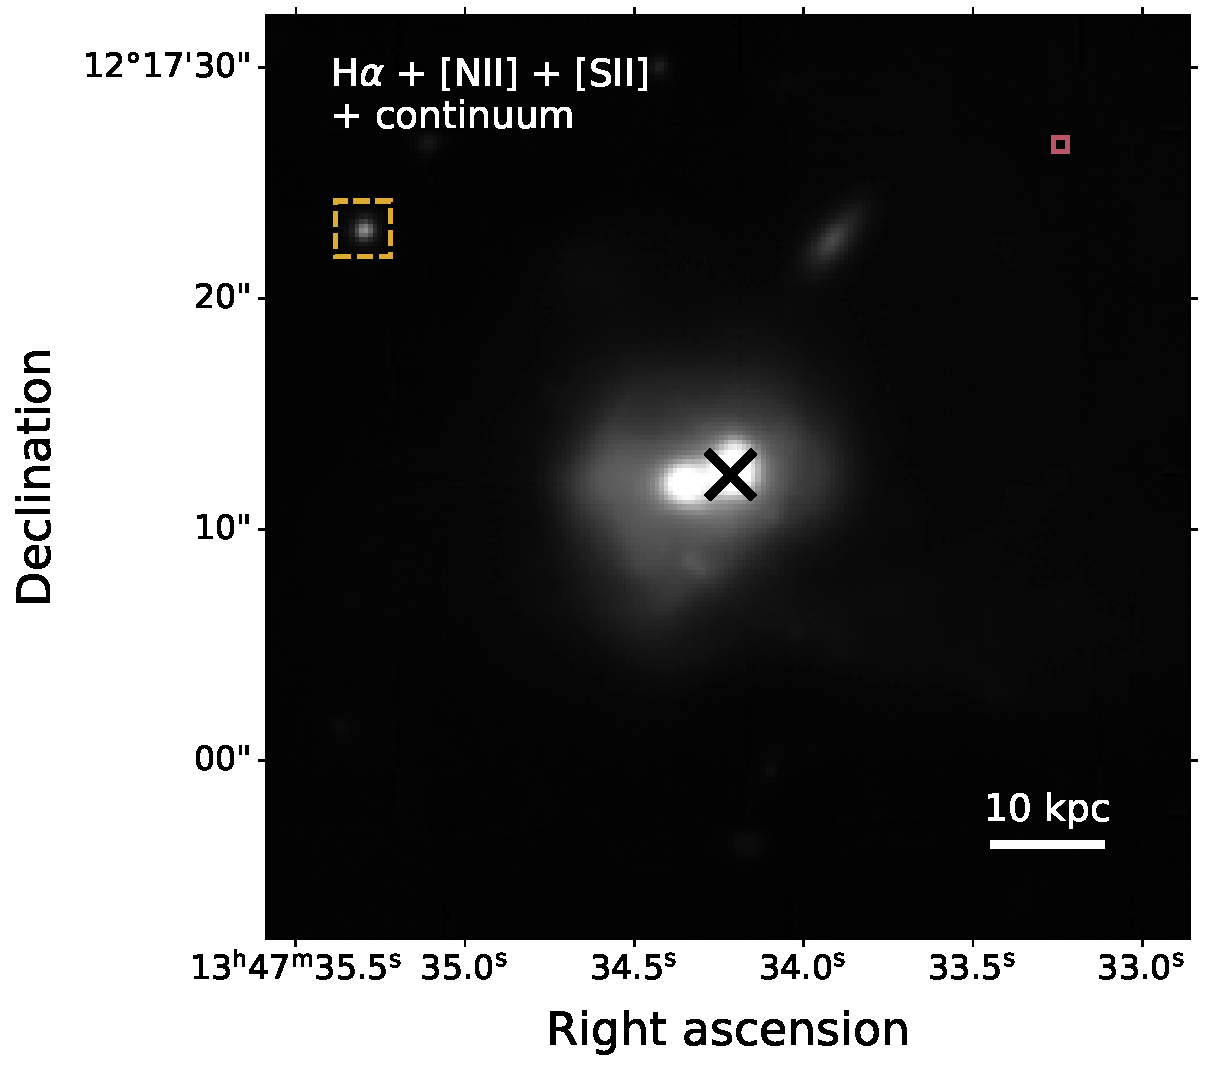
\includegraphics[width=\linewidth]{figures/muse_f13451_1232/f13451_1232_halpha_sii.pdf}
    \caption[H$\alpha$ + {[}NII{]}$\lambda\lambda$6548,6584 + {[}SII{]}$\lambda\lambda$6717,6731 + continuum image of F13451+1232.]{6400--6850\;{\AA} rest-wavelength image (covering H$\alpha$ + [NII]$\lambda\lambda$6548,6584, [SII]$\lambda\lambda$6717,6731, and continuum) of F13451+1232, produced from archival MUSE-DEEP data. The primary nucleus is marked with a black cross, the star used to estimate the atmospheric seeing value of the dataset is marked with a yellow dashed-line box, and the $0.6\times0.6$\;arcsecond region that was extracted for the second-order sky subtraction is marked with a red solid-line box.}
    \label{fig: muse_f13451_1232: observations_and_data_reduction: halpha_sii_image}
\end{figure}

\section{Analysis and results}
\label{section: muse_f13451_1232: analysis_and_results}

\subsection{A Bayesian emission-line fitting routine}
\label{section: muse_f13451_1232: analysis_and_results: bayesian_emission_line_fitting_routine}

In order to fit the large number of emission lines involved in this analysis robustly, I have developed an automated, Bayesian emission-line fitting routine. This routine uses the \textsc{emcee} \textsc{Python} module \citep{FormanMackey2013} --- which is an implementation of the Affine Invariant MCMC Ensemble sampler \citep{Goodman2010} --- to fit a first-order polynomial to the continuum and $N_\mathrm{g}$ Gaussian components to a given emission-line profile. In this routine, $N_\mathrm{g}$ is iteratively increased from zero, and at each iteration, the Bayesian odds of the current and previous iteration are used to determine if another iteration (one more Gaussian component) statistically improves the fit to the line profile, thus preventing over-fitting.

Lines, doublets and emission-line blends (such as H$\alpha$ + {[}NII{]}$\lambda\lambda$6548,6584) were fit individually; a sufficient wavelength range of continuum on either side of the line profile(s) was included in the fits. In cases where the modelled lines arise from a doublet of the same ion (e.g. [SII]$\lambda\lambda$6717,6731), the width of a given Gaussian component was set to be the same for each doublet line, and the wavelength separations were set to those defined by atomic physics \citep{Osterbrock2006}. Furthermore, for lines arising from the same upper energy level, the flux ratios were also set to those defined from atomic physics ([OIII]$(5007/4959)=2.99$; [NII]$(6584/6548)=2.92$: determined with the \textsc{PyNeb Python} module: \citealt{Luridiana2015}).

Before the main production run of the MCMC routine, a burn-in phase was performed. The steps of this phase were not included in determining the final parameters of the fit, as their purpose was to ensure that the walkers started in a region of probability that is more representative of the sampled parameter distribution. 1000 steps were used for both the burn-in and the main production run, as it was found that the walkers converged well before this number of steps; 200 walkers were used in both cases.

The initial starting points for the model parameters were set by Gaussian distributions around physically-motivated estimates: the continuum flux offset (i.e. the $y$-intercept of the first-order polynomial) was set to be the mean flux measured on either side of the emission line; the continuum slope (the gradient of the first-order polynomial) was set to zero; the peak value of each Gaussian component was set as half of the maximum flux value seen in the data, the Gaussian centroids were set to the wavelength of the emission line in the rest frame of the galaxy, and the Gaussian widths were set to be twice the instrumental line width of MUSE ($\sigma_\mathrm{inst}=1.1$\;{\AA}: \citealt{Weilbacher2016}).

Priors for the routine were also physically motivated. For the Gaussian components, their peak values were required to be equal-to or greater-than zero (to ensure only emission was being modelled), their centroids were not allowed to be more than 50\;{\AA} in separation from the rest wavelength of the line in the galaxy's rest frame (corresponding to $v\sim3000$\;km\;s$^{-1}$), and their widths were constrained to be greater than the MUSE instrumental width. Furthermore, the flux ratios for lines arising from the same ions (but with different upper energy levels) were required to be within the ratio limits defined by atomic physics --- for example, 0.44\;\textless\;[SII](6717/6731)\;\textless\;1.45 (determined using the \textsc{PyNeb Python} module). 

The likelihood function used in the MCMC fits was
\begin{equation}
    \chi^2=\frac{1}{2}\mathlarger{\sum^k_{i=1}}\frac{F_\mathrm{\lambda,i}-F^\mathrm{m}_\mathrm{\lambda,i}}{F^\mathrm{err}_\mathrm{\lambda,i}},
    \label{eq: muse_f13451_1232: analysis_and_results: chisq}
\end{equation}
where, at the wavelength step $i$ (and up to the final wavelength step $k$), $F_\mathrm{\lambda,i}$ is the observed flux density, $F^\mathrm{m}_\mathrm{\lambda,i}$ is the  modelled flux density, and ${F^\mathrm{err}_\mathrm{\lambda,i}}$ is the uncertainty associated with the observed flux density.

The fitting routine begins with $N_\mathrm{g}=0$ (i.e. only a first-order polynomial), for which a fit to the data is produced using the MCMC Ensemble. The Bayesian probabilities for the initial run are recorded, and this process is repeated for $N_\mathrm{g}=N_\mathrm{g}+1$ until the ratio of posterior probabilities (Bayesian odds) of successive runs is less than two\footnote{As a check on this criterion, I also performed this routine with the Bayesian Information Criterion (BIC), where the more-complex model was chosen if the difference of BIC values between successive runs was greater than 6. When applied to the MUSE-DEEP data, the resulting model parameters were not significantly different from those produced using the Bayesian odds criterion.}. If this condition is not met, the routine continues until it is fulfilled. In this way, the minimum number of statistically-meaningful Gaussian components required to describe the emission-line profiles is determined by the routine, avoiding over-fitting. 

Cases where only a first-order polynomial was required to adequately describe the spectrum (i.e. $N_\mathrm{g}=0$) were considered to be non-detections, whereas in cases that required one or more Gaussian components, the value for each model parameter was taken to be the 50th percentile for the marginalised probability distribution (i.e. the probability distribution for each parameter), and the $1\sigma$ uncertainties were taken as the 16th and 84th percentiles.

\subsection{The effect of atmospheric seeing on outflow extents and kinematics}
\label{section: muse_f13451_1232: analysis_and_results: seeing}

\subsubsection{Nuclear aperture extraction and modelling}
\label{section: muse_f13451_1232: analysis_and_results: seeing: nuclear_aperture_extraction}

Given that compact ($r$\;\textless\;100\;pc), warm-ionised outflows have been detected and characterised near the primary nucleus of F13451+1232 \citep{Holt2003, Holt2011, Rose2018, Tadhunter2018}, it is possible that the beam-smearing effects of atmospheric seeing have artificially spread this emission to larger spatial scales in the MUSE-DEEP datacube FOV. To account for this, I first extracted a circular aperture centred on the primary nucleus, the radius of which was set to be 0.4\;arcseconds ($\sim$0.9\;kpc), corresponding to the half width at half maximum ($\mathrm{HWHM}=\mathrm{FWHM}/2$) of the seeing value for the dataset (HWHM$_\star=0.40\pm0.10$ arcseconds: Section\;\ref{section: muse_f13451_1232: observations_and_data_reduction: seeing}). This radius was selected because intermediate and broad components of any line profiles within it are expected to be due to the prominent compact outflows \citep{Holt2003, Holt2011}, and there was sufficient signal for the robust modelling and fitting of these profiles. The spaxels contained in the nuclear aperture were summed to give a total nuclear spectrum, while the flux uncertainties of each spaxel were added in quadrature. Second, the Bayesian emission-line-fitting routine described above was used to produce and fit a model to the [OIII]$\lambda\lambda4959,5007$ doublet of the nuclear spectrum. To ensure that the model accounted for the extended blue wings and dual-peaked line profiles seen in the nuclear spectrum, the results of a least-squares fit consisting of three Gaussian components were used as initial parameters for a run of the MCMC line-fitting routine. The resulting model is shown along with the spectrum extracted from the nuclear aperture in Figure\;\ref{fig: muse_f13451_1232: analysis_and_results: seeing: nuclear_aperture_spectrum}, and its parameters are given in Table\;\ref{tab: muse_f13451_1232: analysis_and_results: seeing: nuclear_model}. The two broadest kinematic components of this model  --- henceforth referred to as the `nuclear model' --- are consistent with those of the `broad' and `very broad' components of the nuclear [OIII] fits for F13451+1232 presented by \citet{Rose2018}, and correspond to nuclear outflows. The narrowest component of the nuclear spectrum fit is consistent with the `narrow' component of the \citet{Rose2018} [OIII] model, and its kinematics correspond to those of the kpc-scale disk detected in CO(1--0) emission in Chapter\;\ref{chapter: alma_f13451_1232} (see also \citealt{Lamperti2022}). Note that while the fit to the nuclear spectrum does not precisely describe the details of the emission-line profile, it is adequate for the purposes of this study.

\subsubsection{Emission-line fits of the extended emission}
\label{section: muse_f13451_1232: analysis_and_results: seeing: extended_emission_fits}

To determine the large-scale warm-ionised gas kinematics, for each spaxel in the deep datacube, the Bayesian emission-line fitting routine was used to fit a model consisting of the nuclear model (accounting for beam-smeared, nuclear-outflow emission) and $N_\mathrm{g}$ additional Gaussian components (accounting for genuine, non-beam-smeared emission) to the [OIII]$\lambda\lambda$4959,5007 doublet. The centroid wavelengths, widths and relative intensities of the Gaussian components of the nuclear model were fixed; only the peak flux density was allowed to vary. In this way, the line-fitting routine was able to determine the extent to which the nuclear-outflow emission was smeared across the MUSE field of view, as well as detect and isolate the contributions of genuine extended emission to line profiles in each spaxel. Similar approaches to PSF-subtraction and beam-smearing-correction have been taken by previous studies (e.g. \citealt{Carniani2015, Kakkad2020, Speranza2024}), although here, only broad components (FWHM\;\textgreater\;500\;km\;s$^{-1}$) are included in the nuclear model.


\begin{table}
    \renewcommand{\arraystretch}{1.2}
    \centering
    \begin{tabular}{ccccc}
    Peak flux density     &   Centroid   &  Velocity  & FWHM & FWHM \\
    ($\times10^{-16}$\;\AA) &    wavelength (\AA)  &   shift (km\;s$^{-1}$) & (\AA) & (km\;s$^{-1}$) \\
    \hline \\
    $3.52\pm0.34$  &   $5608.9\pm0.8$   &  $-382.2\pm43.9$  &  $18.8\pm0.8$ &  $1006.1\pm42.8$  \\
    $1.46\pm0.06$  &   $5592.7\pm0.7$   &  $-1248.2\pm35.9$  &  $53.1\pm1.3$ &  $2846.7\pm68.1$  \\
    $1.05\pm0.37$  &   $5615.8\pm0.9$   & $-19.5\pm47.5$ &  $7.7\pm3.8$ & $412.9\pm203.5$  \\
    \end{tabular}
    \caption[Parameters for the {[}OIII{]}$\lambda\lambda4959,5007$ model derived from a circular aperture around the primary nucleus of F13451+1232 in the MUSE-DEEP data.]{Parameters for the [OIII] model derived from fitting the spectrum extracted from a circular aperture of radius $r=0.4$\;arcseconds around the primary nucleus of F13451+1232. The presented velocity shifts are relative to the galaxy rest frame, and the FWHM values have been corrected for instrumental broadening. The `nuclear model' referred to in this work consists of the two broadest components presented here (the top two rows); the narrowest component (bottom row) is kinematically distinct, and corresponds to the kpc-scale disk in the nucleus of F13451+1232 (see Chapter\;\ref{chapter: alma_f13451_1232}).}
    \label{tab: muse_f13451_1232: analysis_and_results: seeing: nuclear_model}
\end{table}

\begin{figure}[!ht]
    \centering
    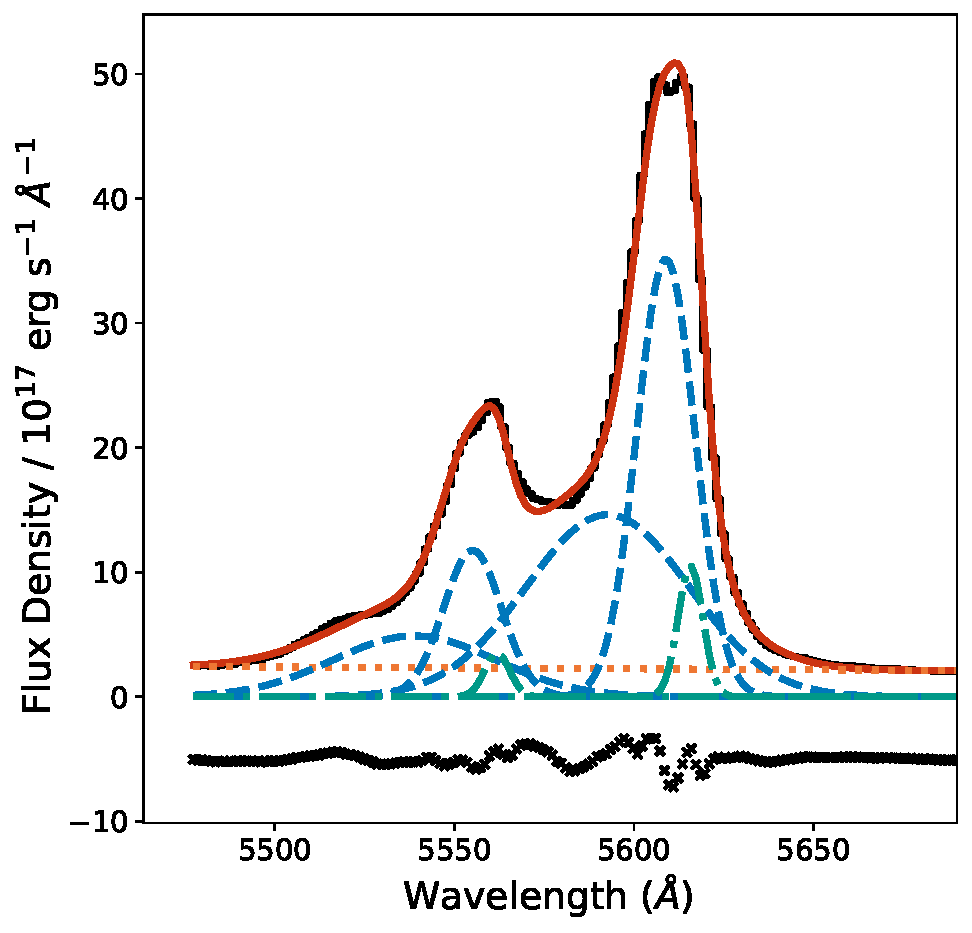
\includegraphics[width=0.7\linewidth]{figures/muse_f13451_1232/nuclear_model.pdf}
    \caption[{[}OIII{]}$\lambda\lambda$4959,5007 line profile (and nuclear model fit) for the primary nucleus of F13451+1232]{[OIII]$\lambda\lambda$4959,5007 line profile for the extracted circular $r=0.4$\;arcsec aperture centred on the primary nucleus of F13451+1232 (black solid line). The overall fit to the line profile is shown as a solid red line; the broad Gaussian components of this fit (the `nuclear model') are shown as dashed blue lines, the narrow Gaussian component is shown as a dash-dotted green line, and the first-order polynomial (accounting for the continuum) is shown as a dotted orange line. Residuals (flux $-$ model) are shown as crosses below the line profile.}
    \label{fig: muse_f13451_1232: analysis_and_results: seeing: nuclear_aperture_spectrum}
\end{figure}

\subsubsection{Beam smearing of compact outflow emission}
\label{section: muse_f13451_1232: analysis_and_results: seeing: psf}

As a measure of the extent of beam smearing of the compact nuclear-outflow emission, in the left panels of Figure\;\ref{fig: muse_f13451_1232: analysis_and_results: seeing: nuclear_model_psf} I present the spatial distribution of the peak flux intensity of the nuclear model in the central $7\times7$\;arcsecond region around the primary nucleus of F13451+1232, as determined by fitting the [OIII]$\lambda\lambda4959,5007$ doublet in each spaxel. The flux of the nuclear-model components appears to be radially symmetric around the location of the primary nucleus, indicative of beam smearing. To investigate this further, a two-dimensional Moffat profile was fit to the spatial flux distribution of the nuclear model, which is shown along with residuals (the flux of the fitted two-dimensional Moffat profile subtracted from the peak flux of the nuclear model) in Figure\;\ref{fig: muse_f13451_1232: analysis_and_results: seeing: nuclear_model_psf} --- it can be seen that the spatial distribution of the nuclear-model flux is well described by a Moffat profile of $\mathrm{FWHM}=0.74\pm0.02$ arcseconds. This value is consistent (within $1\sigma$) with the seeing value measured from a star in the MUSE-DEEP data FOV ($\mathrm{FWHM}_\star=0.79\pm0.10$\;arcseconds: Section\;\ref{section: muse_f13451_1232: observations_and_data_reduction: seeing}; see Figure\;\ref{fig: muse_f13451_1232: observations_and_data_reduction: halpha_sii_image}), providing direct evidence that atmospheric seeing artificially spread emission from the nuclear outflows across the MUSE FOV.

\begin{figure}[!t]
    \begin{subfigure}[t]{0.3355\linewidth}
        \centering
        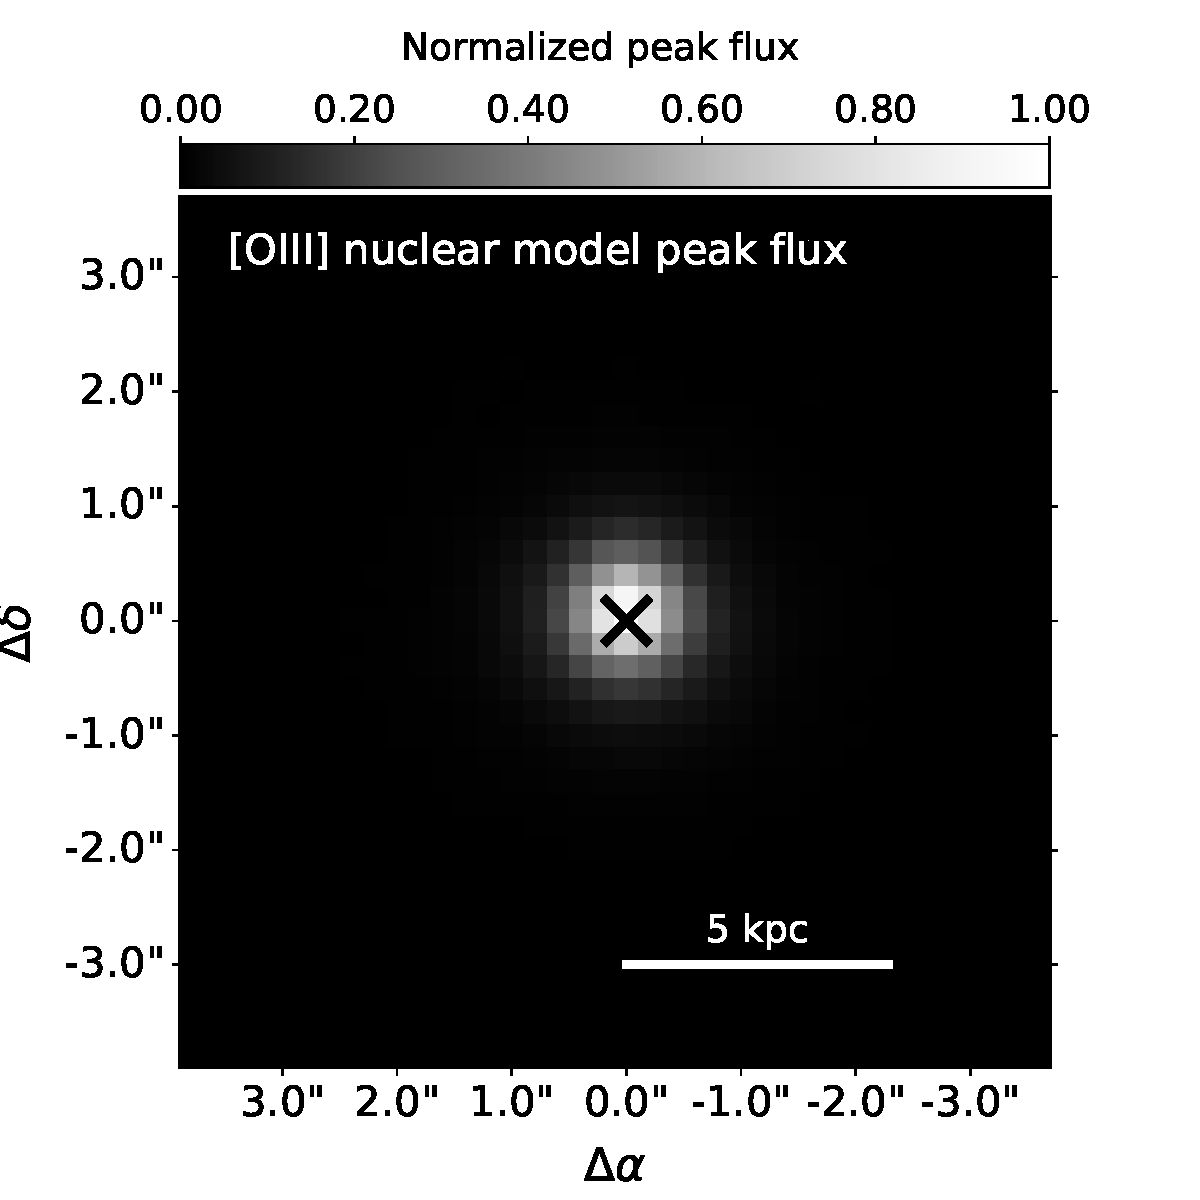
\includegraphics[width=\textwidth, trim={0 0 1.5cm 0}, clip]{figures/muse_f13451_1232/nuclear_model_psf.pdf}
    \end{subfigure}
    \hspace*{\fill}
    \begin{subfigure}[t]{0.3\linewidth}
        \centering
        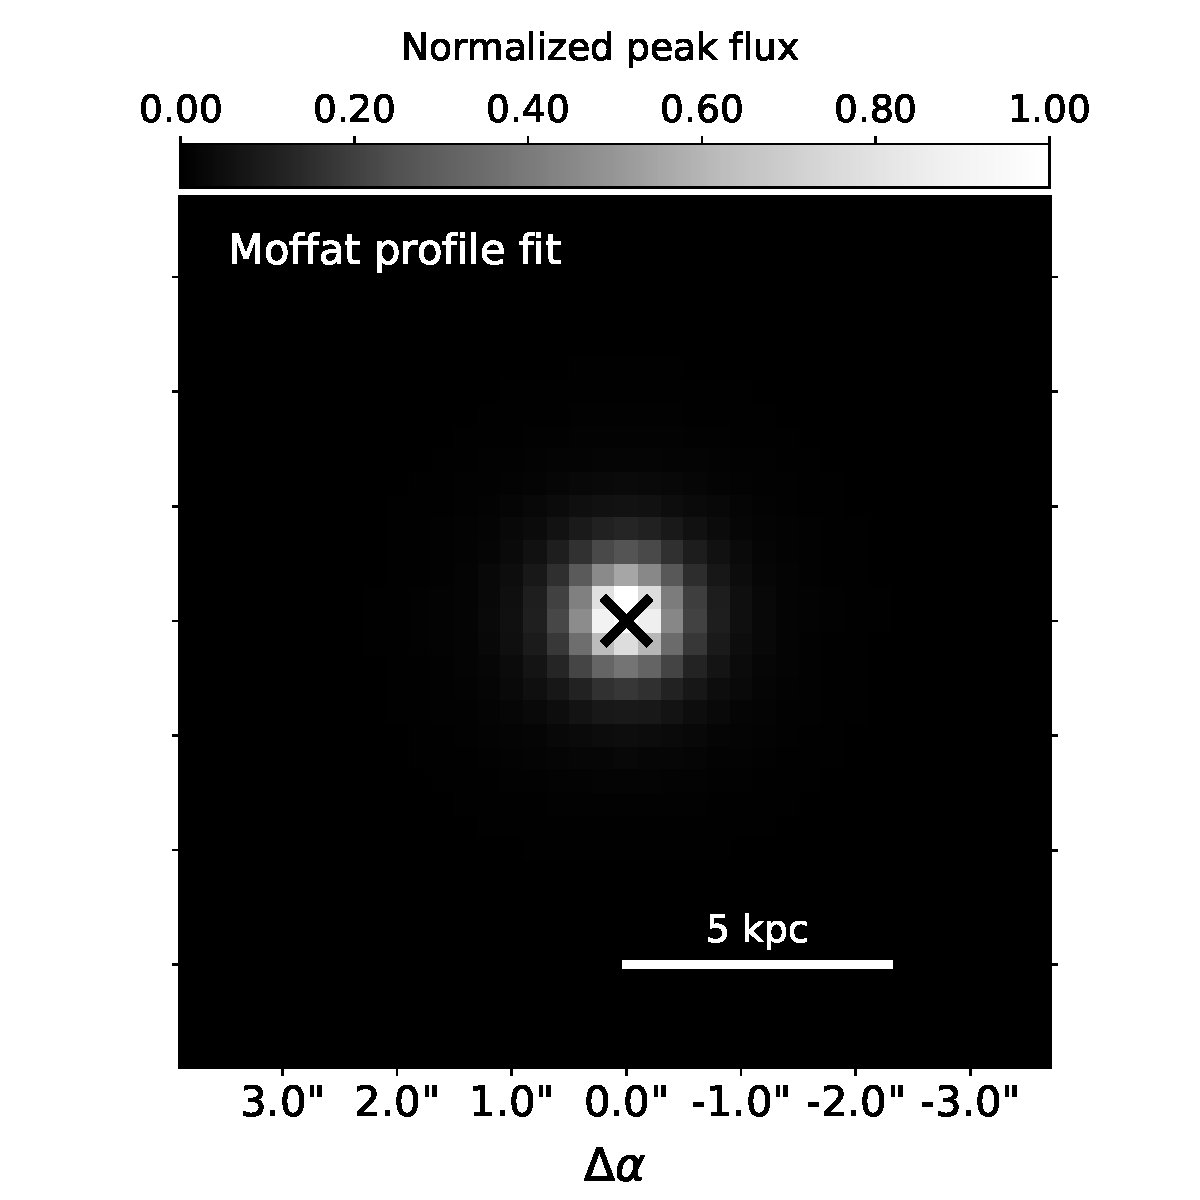
\includegraphics[width=\textwidth, trim={2cm 0 1.5cm 0}, clip]{figures/muse_f13451_1232/nuclear_model_psf_model.pdf}
    \end{subfigure}
    \hspace*{\fill}
    \begin{subfigure}[t]{0.3\linewidth}
        \centering
        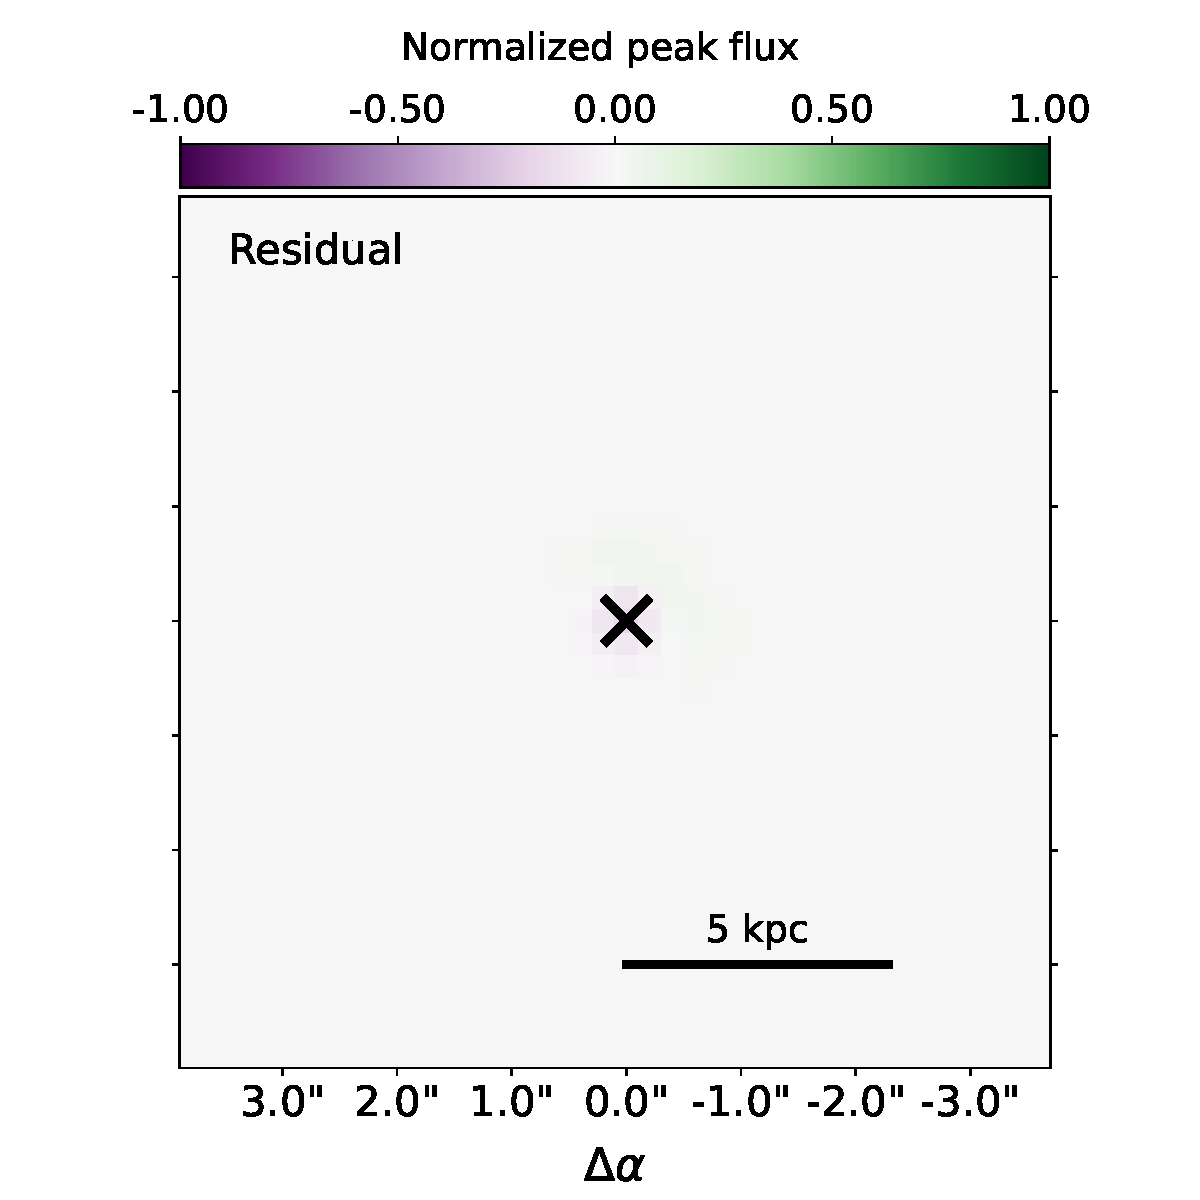
\includegraphics[width=\textwidth, trim={2cm 0 1.5cm 0}, clip]{figures/muse_f13451_1232/nuclear_model_psf_residual.pdf}
    \end{subfigure} \\
    \begin{subfigure}[t]{0.3355\linewidth}
        \centering
        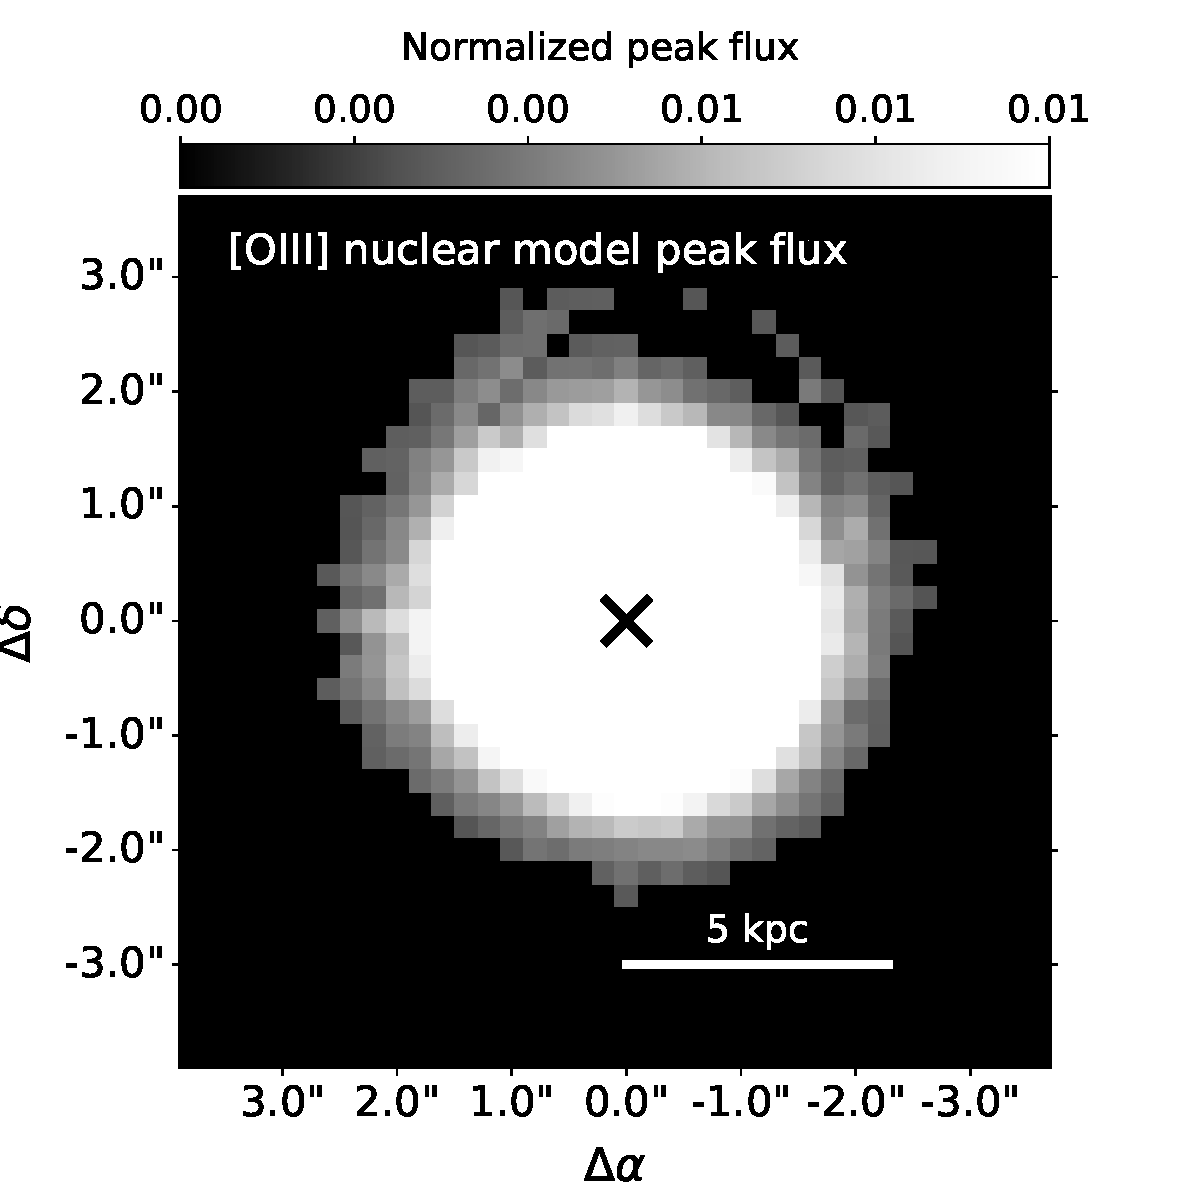
\includegraphics[width=\textwidth, trim={0 0 1.5cm 0}, clip]{figures/muse_f13451_1232/nuclear_model_psf_highcrop.pdf}
    \end{subfigure}
    \hspace*{\fill}
    \begin{subfigure}[t]{0.3\linewidth}
        \centering
        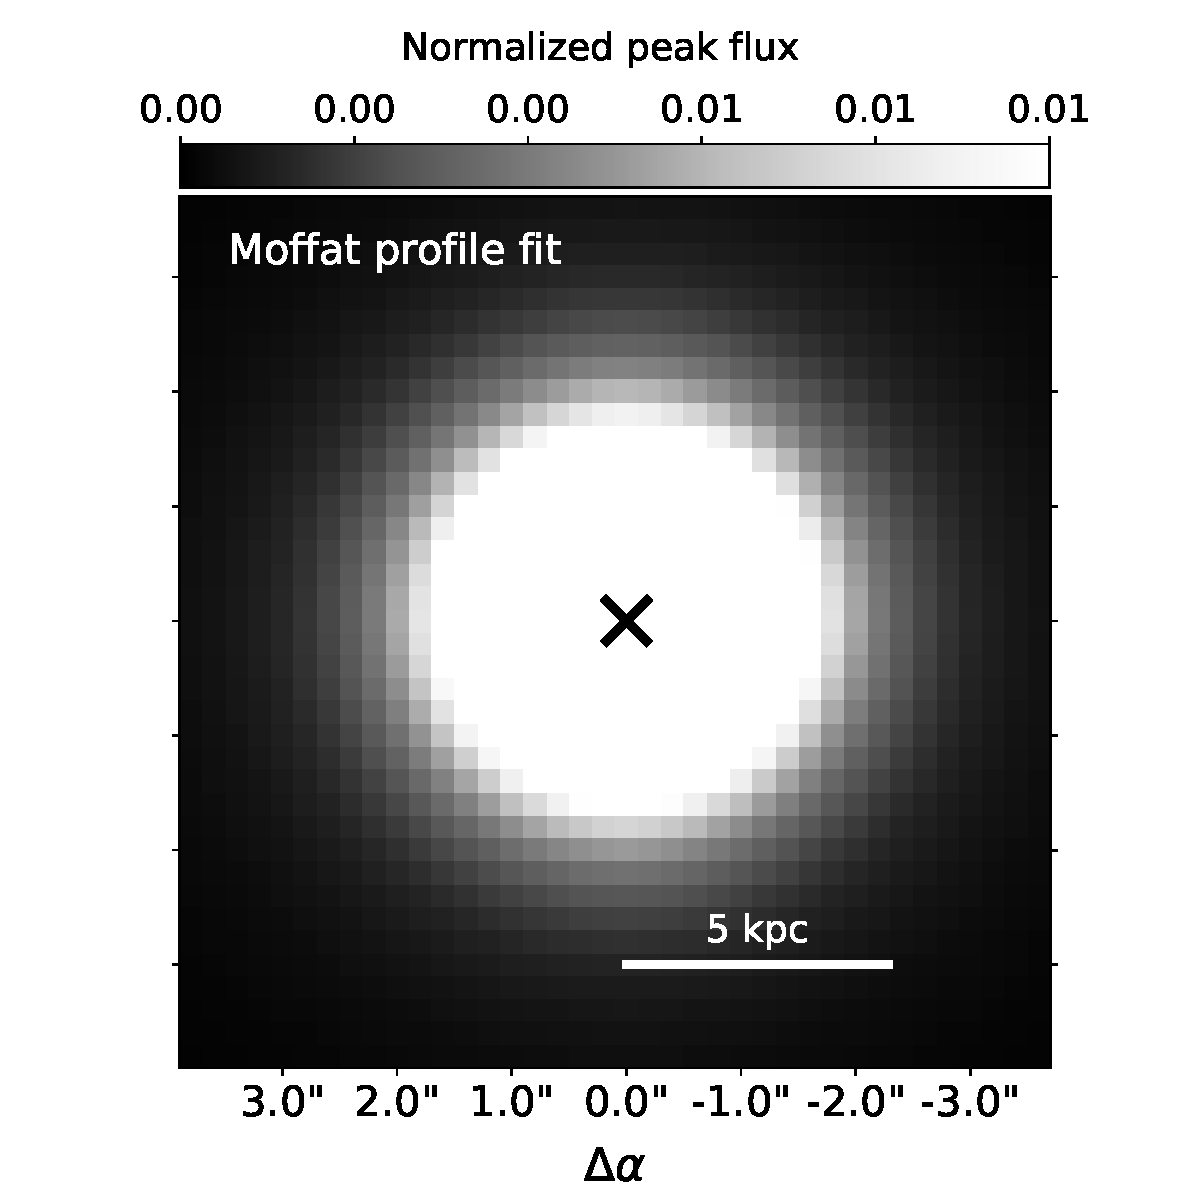
\includegraphics[width=\textwidth, trim={2cm 0 1.5cm 0}, clip]{figures/muse_f13451_1232/nuclear_model_psf_model_highcrop.pdf}
    \end{subfigure}
    \hspace*{\fill}
    \begin{subfigure}[t]{0.3\linewidth}
        \centering
        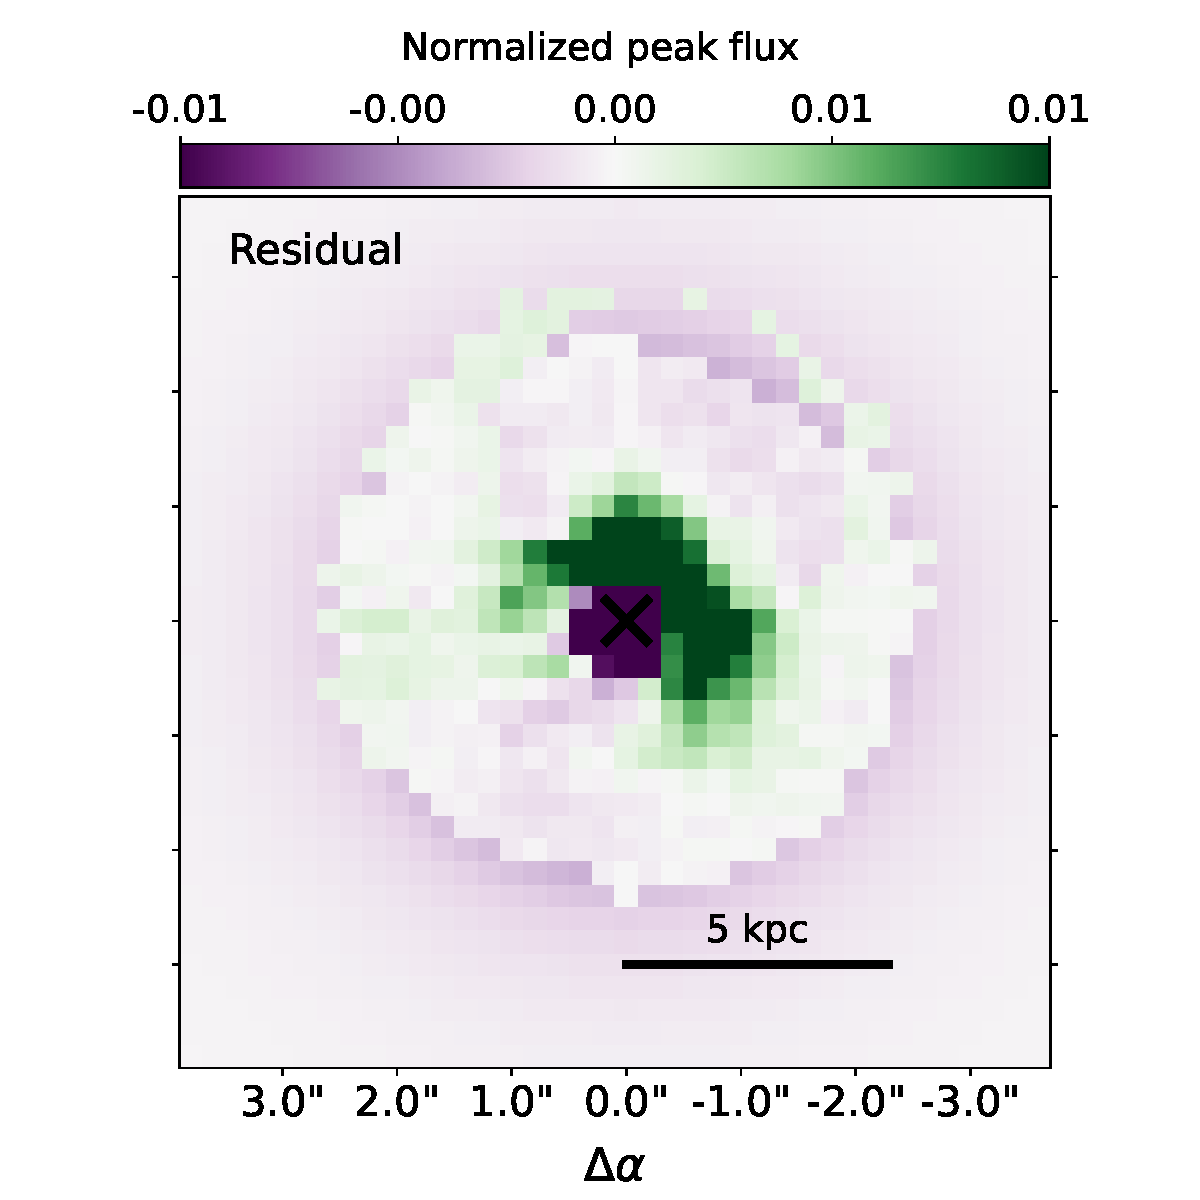
\includegraphics[width=\textwidth, trim={2cm 0 1.5cm 0}, clip]{figures/muse_f13451_1232/nuclear_model_psf_residual_highcrop.pdf}
    \end{subfigure}
    \caption[The spatial distribution of the peak flux of the {[}OIII{]} nuclear model, a two-dimensional Moffat profile fit to this distribution, and the residuals of this fit in the inner 7\;arcseconds (15\;kpc) of the primary nucleus of F13451+1232.]{The spatial distribution of the peak flux of the nuclear model in the [OIII] fits (left panel), the results of two-dimensional Moffat profile fits to this distribution (middle panel), and residuals ([OIII] nuclear model peak flux $-$ model; right panel) in the inner 7\;arcseconds (15\;kpc) of the primary nucleus of F13451+1232 (marked with a black cross). The flux in all cases is normalised to the highest flux value of the nuclear model (upper left panel); the top row shows the full range of normalised flux, while the bottom row shows a significantly reduced range for presentation purposes. It can be seen that the [OIII]-nuclear-model flux is well-described by a Moffat profile with an FWHM of $0.74\pm0.02$\;arcseconds.}
    \label{fig: muse_f13451_1232: analysis_and_results: seeing: nuclear_model_psf}
\end{figure}


\begin{figure}[!t]
    \begin{subfigure}[]{0.51\linewidth}
        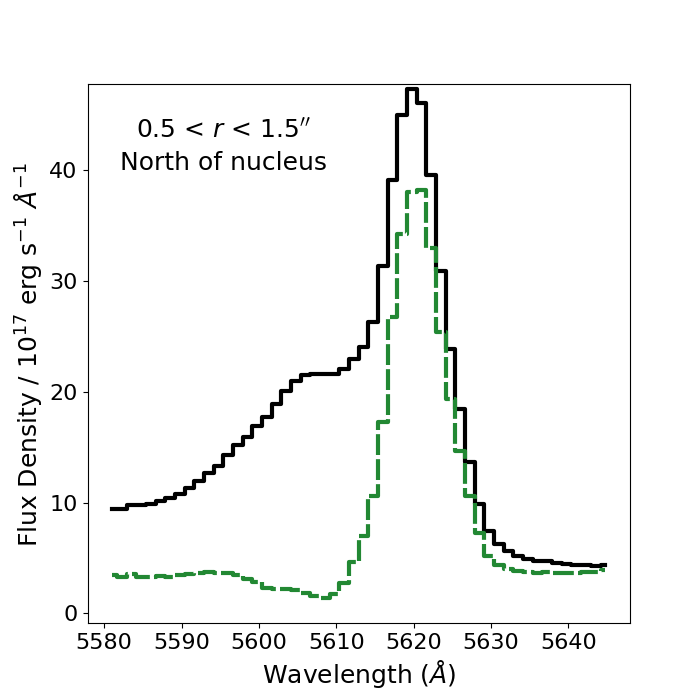
\includegraphics[width=\linewidth, trim={0 1.8cm 0 0}, clip]{figures/muse_f13451_1232/broadsub_apertures/ap1_original_broadsub_comparison.png}
    \end{subfigure}
    \hfill
    \begin{subfigure}[]{0.48\linewidth}
        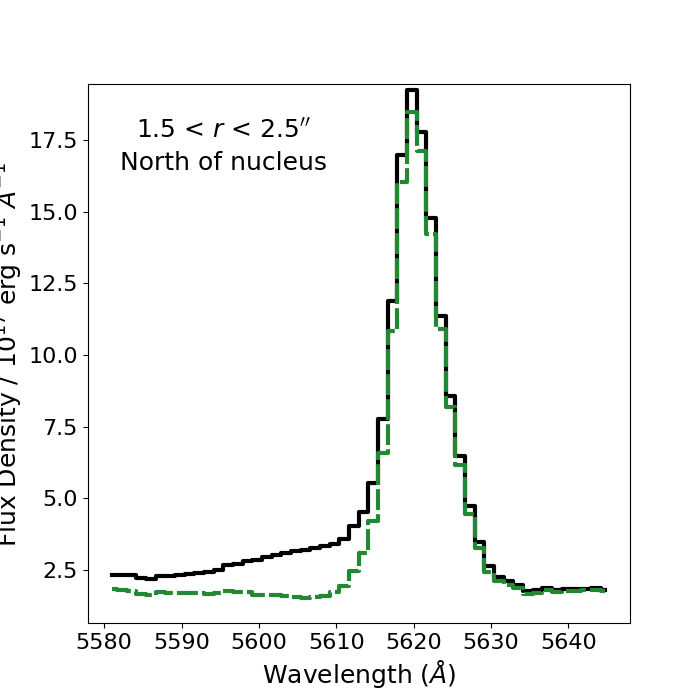
\includegraphics[width=\linewidth, trim={1.1cm 1.8cm 0 0}, clip]{figures/muse_f13451_1232/broadsub_apertures/ap2_original_broadsub_comparison.png}
    \end{subfigure}
    \begin{subfigure}[]{0.51\linewidth}
        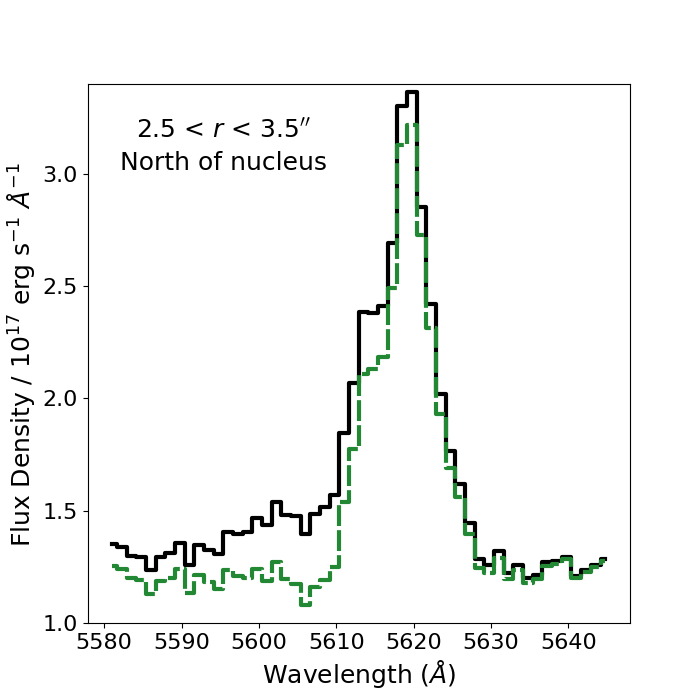
\includegraphics[width=\linewidth, trim={0 0 0 1.5cm}, clip]{figures/muse_f13451_1232/broadsub_apertures/ap3_original_broadsub_comparison.png}
    \end{subfigure}
    \hfill
    \begin{subfigure}[]{0.48\linewidth}
        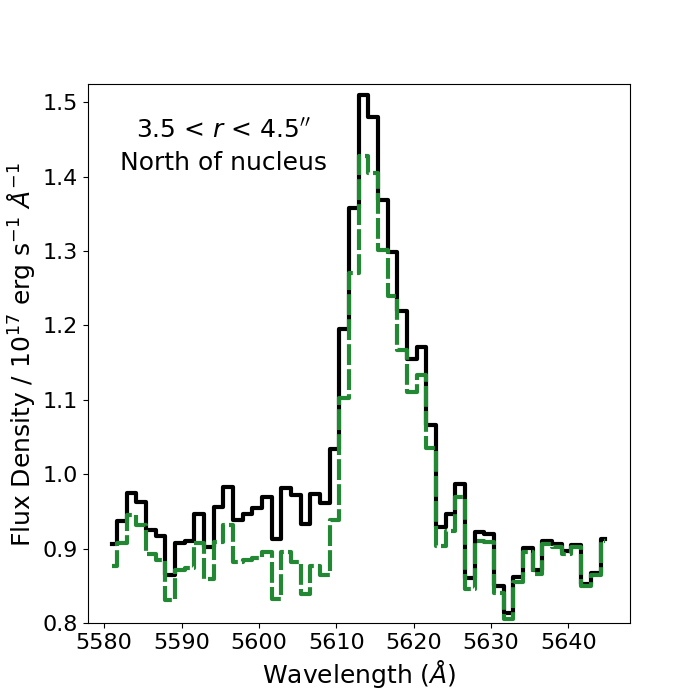
\includegraphics[width=\linewidth, trim={1.1cm 0 0 1.5cm}, clip]{figures/muse_f13451_1232/broadsub_apertures/ap4_original_broadsub_comparison.png}
    \end{subfigure}
    \caption[{[}OIII{]}$\lambda$5007 line profiles extracted from apertures at increasing radial distances north of the primary nucleus of F13451+1232, for cases in which beam smearing of nuclear emission is and is-not accounted for.]{[OIII]$\lambda5007$ line profile extracted from rectangular $2\times1$\;arcsecond apertures (centred on the primary nucleus in the east-west direction) at increasing radial distances (labelled) to the north of the nucleus, for the original datacube (solid black line) and the datacube with the nuclear model subtracted using a Moffat distribution (dashed green line). It can be seen that the beam-smeared nuclear outflow emission is significant between 5595\;\textless\;$\lambda$\;\textless\;5610\;{\AA} ($-1200$\;\textless\;$v$\;\textless\;$-420$\;km\;s$^{-1}$) in all apertures.}
    \label{fig: muse_f13451_1232: analysis_and_results: seeing: broadsub_line_profile_comparison}
\end{figure}

To investigate the residual emission after the beam-smeared nuclear-outflow emission has been accounted for, I subtracted the [OIII] nuclear model from each spaxel of the datacube. This was done by first normalising the peak flux of the nuclear model to unity, multiplying it by the value of the Moffat profile fit to the [OIII] nuclear model flux distribution in each spaxel (middle panels of Figure\;\ref{fig: muse_f13451_1232: analysis_and_results: seeing: nuclear_model_psf}; which is consistent with what is expected from atmospheric seeing, as noted above), and subtracting this from the original datacube. To demonstrate the radial extent to which the beam-smeared emission contributes significantly to the line profiles, I extracted a series of rectangular $2\times1$\;arcsecond apertures --- centred on the nucleus in the east-west direction --- at increasing radial distances north of the nucleus from this datacube and the original datacube. I present the [OIII]$\lambda5007$ line profiles in these apertures for both datacubes in Figure\;\ref{fig: muse_f13451_1232: analysis_and_results: seeing: broadsub_line_profile_comparison}, which demonstrate that the beam-smeared nuclear-outflow emission contributes significantly to the flux between 5595\;\textless\;$\lambda$\;\textless\;5610\;{\AA} ($-1200$\;\textless\;$v$\;\textless\;$-420$\;km\;s$^{-1}$) in all apertures, including in an aperture that covers a radial extent of 3.5\;\textless\;$r$\;\textless\;4.5\;arcseconds north of the primary nucleus.

As further confirmation that beam smearing is responsible for the spatial extent of the broad [OIII] emission, a series of annuli were extracted from both around the primary nucleus of F13451+1232 and the star in the MUSE-DEEP FOV that was used to measure the seeing in Section\;\ref{section: muse_f13451_1232: observations_and_data_reduction: seeing}. In both cases, the annuli were centred on the brightest pixel of the flux distribution and had fixed widths of ${\Delta}r=0.5$\;arcseconds; the inner radius of the annuli was increased in 0.5\;arcsecond steps from $r=0.0$\;arcseconds to 2.0\;arcseconds. The pixels in each annulus around the primary nucleus of F13451+1232 were summed (and uncertainties added in quadrature) to produce a spectrum, to which the nuclear model + $N_g$ Gaussian components + first-order polynomial was fit. The normalised flux in each annulus, relative to the flux level of the innermost annulus (i.e. a circular aperture of radius $r=0.5$\;arcseconds), is shown for both the peak flux of these nuclear model fits and the monochromatic [OIII] flux of the star in Figure\;\ref{fig: muse_f13451_1232: analysis_and_results: seeing: star_outflow_annuli}. With the exception of the 0.5\;\textless\;$r$\;\textless\;1.0\;arcsecond annulus, the flux distribution of the nuclear model closely follows that of the star (and therefore the PSF of the seeing disk). The discrepancy in flux in the 0.5\;\textless\;$r$\;\textless\;1.0\;arcsecond (1.1\;\textless\;$r$\;\textless\;2.2\;kpc) annulus can be explained as genuine intermediate-velocity emission from the host galaxy system (consistent with what is expected in a merger) contributing to the line profiles on these scales. Overall, this is further strong evidence that beam-smeared compact-outflow emission can be significant up to at least a radial distance of 2.5\;arcseconds --- six times the HWHM of the seeing disk ($\mathrm{HWHM}_\star=0.40\pm0.10$\;arcseconds).

\begin{figure}[!h]
    \vspace*{0.8cm}
    \centering
    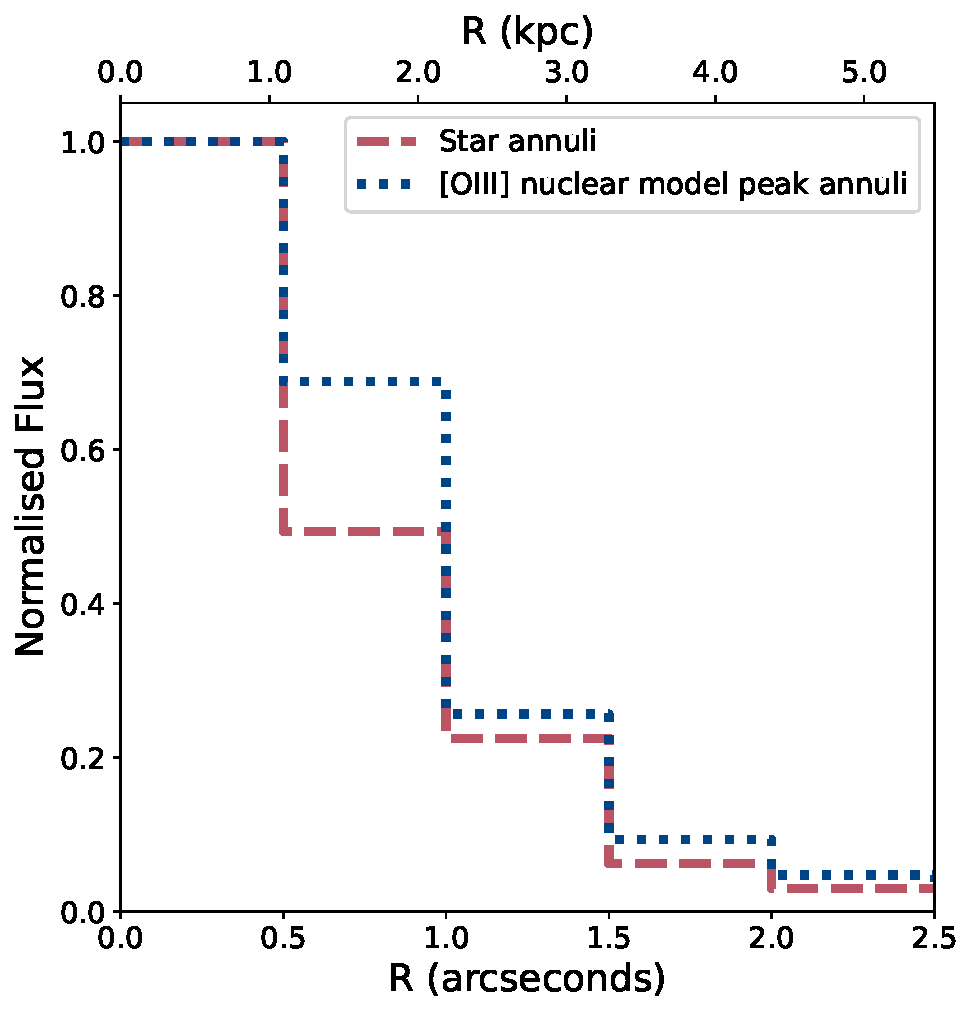
\includegraphics[width=0.7\linewidth]{figures/muse_f13451_1232/star_outflow_annuli.pdf}
    \caption[Normalized fluxes in concentric apertures taken from \textbf{1)} the peak flux of the {[}OIII{]} nuclear model fits around the primary nucleus of F13451+1232 and \textbf{2)} the {[}OIII{]} flux of a star in the FOV of the MUSE DEEP dataset.]{Peak flux values of nuclear-model fits to spectra extracted from annuli around the primary nucleus of F13451+1232 (dotted blue line), and the total monochromatic [OIII] flux of the pixels in each annulus around a star in the field of view of the MUSE observations (red dashed line); the fluxes have been normalised to the value of the innermost annulus in both cases. With the exception of the 0.5\;\textless\;$r$\;\textless\;1.0\;arcsecond annulus --- which likely also contains real intermediate-velocity emission from the host galaxy/merger --- the normalised-flux profiles are similar, indicating that the spatial extent of the broad lines around the primary nucleus is due to the beam smearing of nuclear-outflow emission.}
    \label{fig: muse_f13451_1232: analysis_and_results: seeing: star_outflow_annuli}
\end{figure}

\subsubsection{Accounting for atmospheric seeing in velocity maps}
\label{section: muse_f13451_1232: analysis_and_results: seeing: velocity_maps}

In order to determine the impact of the beam-smeared nuclear-outflow emission on measurements of outflow radial extents and kinematics, the fitting procedure was repeated as outlined in Sections \ref{section: muse_f13451_1232: analysis_and_results: bayesian_emission_line_fitting_routine} and \ref{section: muse_f13451_1232: analysis_and_results: seeing: nuclear_aperture_extraction} for every spaxel in the cube, but the nuclear model was not included in the fits. This is henceforth referred to as the `free-fitting' case, and was done to provide a test of what would be found if the beam smearing of the nuclear-outflow emission had not been accounted for.

$W_\mathrm{80}$ ($v_\mathrm{90}-v_\mathrm{10}$: Section\;\ref{section: introduction: outflows: kinematics_and_geometry: kinematics}) maps were created for the results of both line-fitting approaches (i.e including the nuclear-model Gaussian components, and the free fits). To create the $W_\mathrm{80}$ maps, first, any spaxels for which the peak flux density value of the highest-flux Gaussian component was less than $1\sigma_\mathrm{std}$ from the continuum were not considered. In the free-fitting case, all Gaussian components were used to measure $W_\mathrm{80}$, while in the fits that included the nuclear model, only the additional (non-nuclear-model) Gaussian components were used. For each case, the total fluxes of the Gaussian components involved were calculated, and the $v_\mathrm{90}$ and $v_\mathrm{10}$ percentile velocities (the velocities containing 90 and 10\;per\;cent of the total line flux, respectively) were determined following the method described in Section\;\ref{section: xshooter_ic5063: properties_of_outflowing_gas: uvb_vis_analysis_and_results: kinematics} (see also \citealt{Rose2018}). These percentile velocities were then used to calculate the $W_\mathrm{80}$ parameter. The resulting maps for the inner $6\times6$\;arcsecond region around the primary nucleus are shown in Figure\;\ref{fig: muse_f13451_1232: analysis_and_results: extended_emission: w80_maps}. Furthermore, flux-weighted velocity shifts ($v_w$) in each spaxel for both cases were determined using Equation \ref{eq: xshooter_ic5063: flux_velocity} (see also \citealt{Rose2018}); these maps are presented in Figure\;\ref{fig: muse_f13451_1232: analysis_and_results: extended_emission: vw_maps}.

\begin{figure*}
    \centering
    \begin{subfigure}[b]{0.5175\linewidth}        
        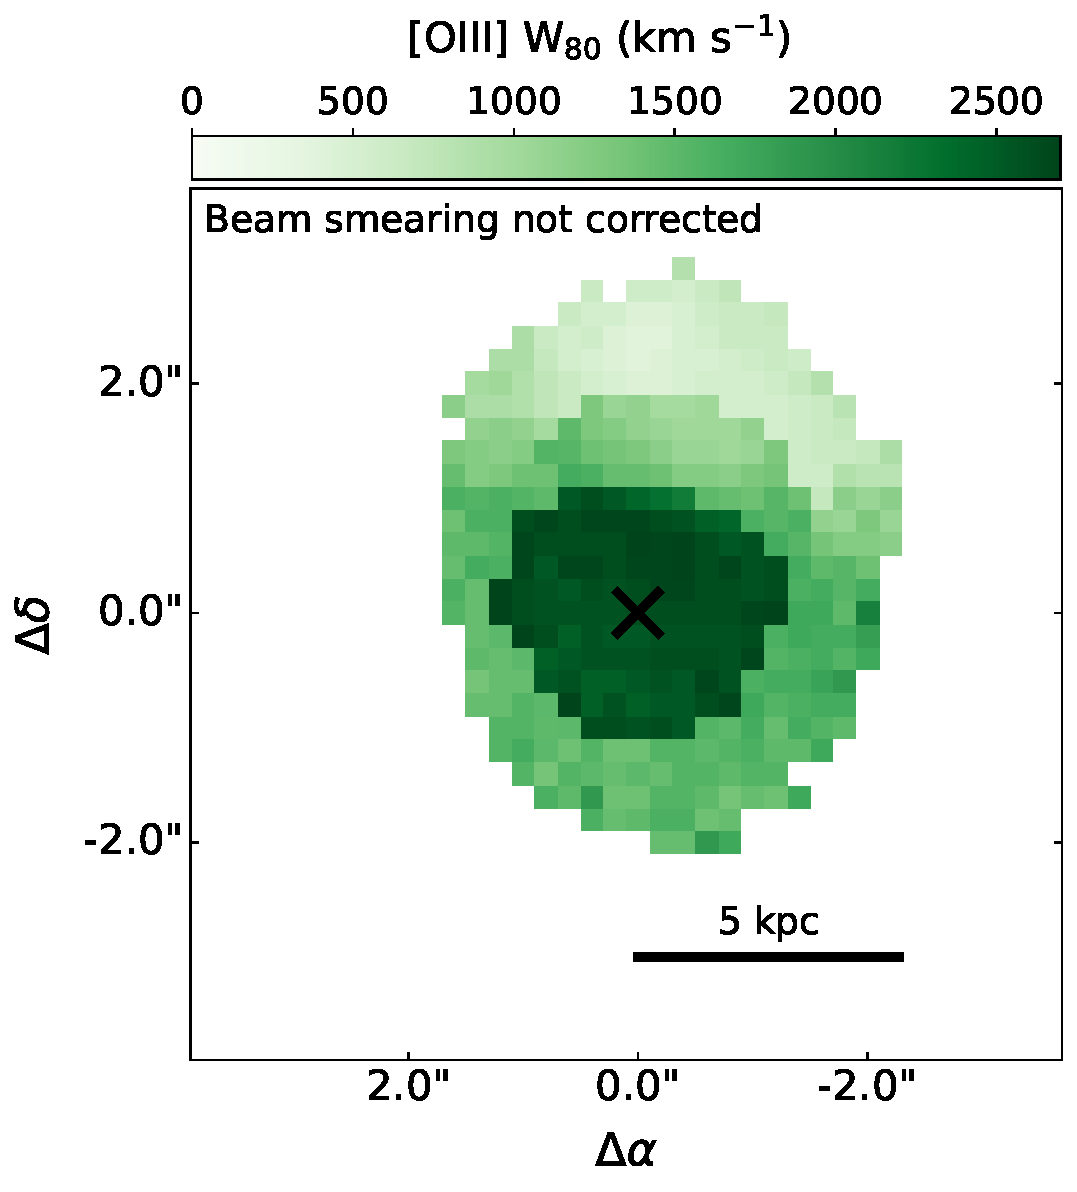
\includegraphics[width=\textwidth]{figures/muse_f13451_1232/w80_map_free.pdf}
    \label{fig: muse_f13451_1232: analysis_and_results: extended_emission: w80_map_free}
    \end{subfigure}
    \hfill
    \begin{subfigure}{0.43\linewidth}        
        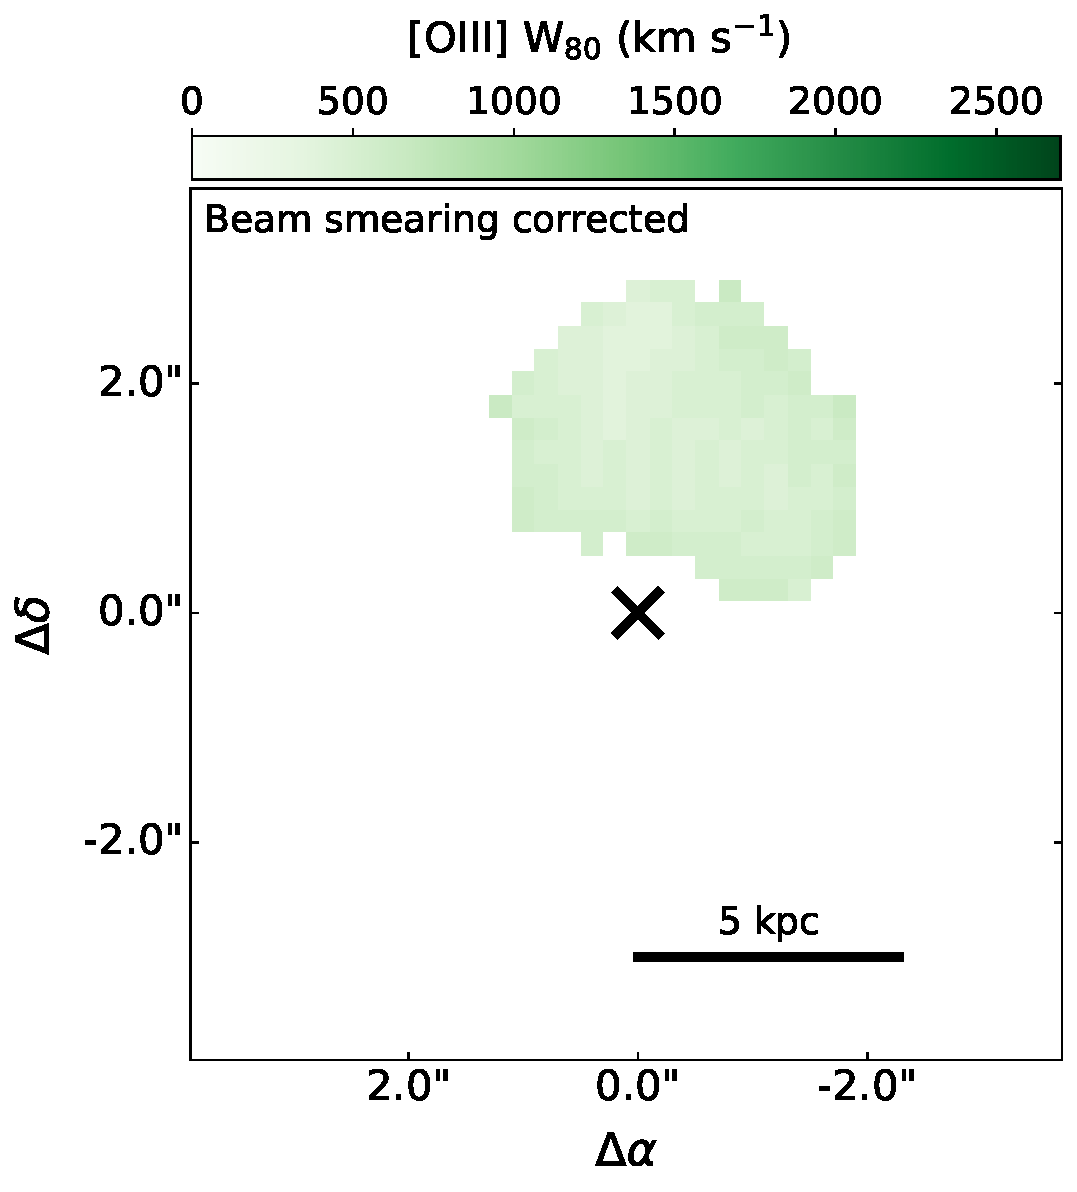
\includegraphics[width=\linewidth, trim={3.1cm 0 0 0}, clip]{figures/muse_f13451_1232/w80_map_nm.pdf}
    \label{fig: muse_f13451_1232: analysis_and_results: extended_emission: w80_map_nm}
    \end{subfigure}
    \caption[Beam-smearing-corrected and non-beam-smearing-corrected $W_\mathrm{80}$ velocity-width maps of the central $6\times6$\;arcsecond ($13\times13$\;kpc) region around the primary nucleus of F13451+1232.]{Non-parametric velocity width ($W_\mathrm{80}=v_\mathrm{90}-v_\mathrm{10}$) maps of the central $6\times6$\;arcsecond ($13\times13$\;kpc) region around the primary nucleus of F13451+1232 (black cross), as measured from free-fitting Gaussian components (left panel) and fitting the nuclear model and $N_\mathrm{g}$ Gaussian components (in which only the $N_\mathrm{g}$ Gaussian components were used to measure $W_\mathrm{80}$; right panel). The former case (left panel) is what would be expected had the beam smearing of compact high-velocity outflow emission not been accounted for, while the latter case (right panel) accounts for this beam smearing.}
    \label{fig: muse_f13451_1232: analysis_and_results: extended_emission: w80_maps}
    \vspace*{12pt}
    \centering
    \begin{subfigure}[b]{0.5175\linewidth}        
        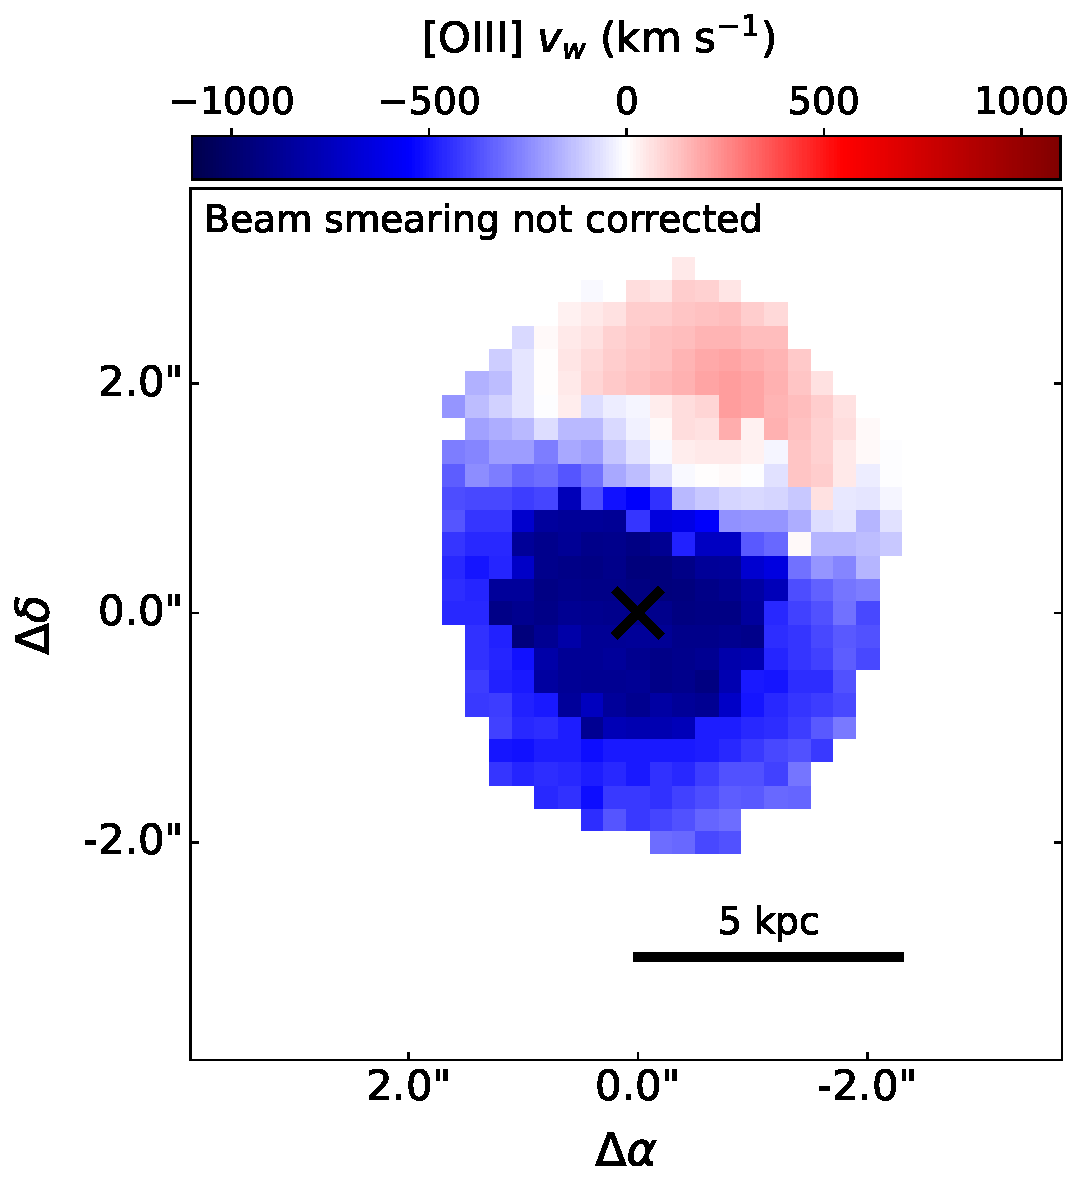
\includegraphics[width=\textwidth]{figures/muse_f13451_1232/vw_map_free.pdf}
    \label{fig: muse_f13451_1232: analysis_and_results: extended_emission: vw_map_free}
    \end{subfigure}
    \hfill
    \begin{subfigure}{0.43\linewidth}        
        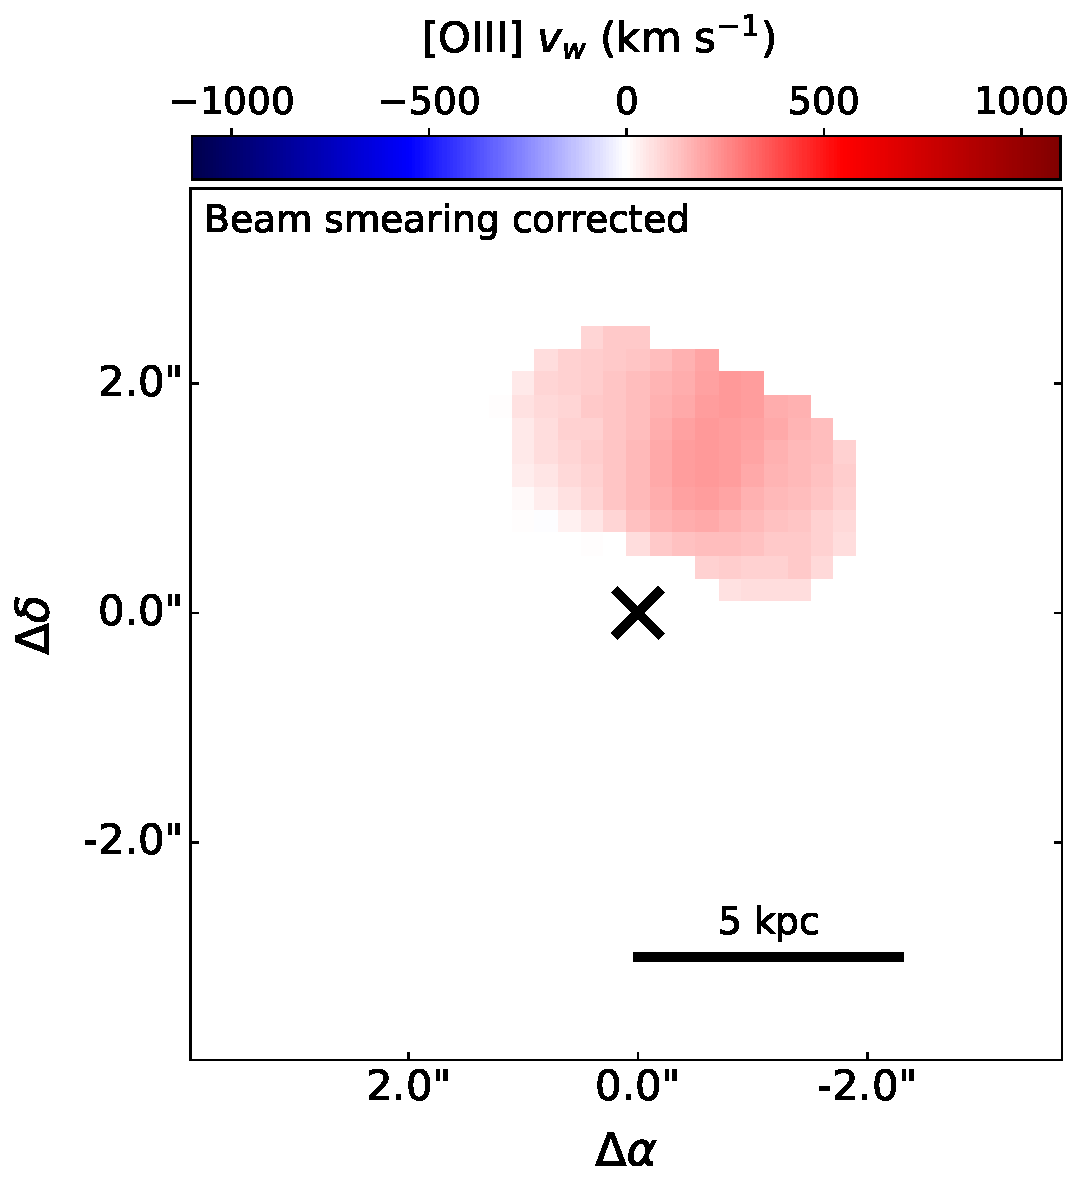
\includegraphics[width=\linewidth, trim={3.1cm 0 0 0}, clip]{figures/muse_f13451_1232/vw_map_nm.pdf}
    \label{fig: muse_f13451_1232: analysis_and_results: extended_emission: vw_map_nm}
    \end{subfigure}
    \caption[Beam-smearing-corrected and non-beam-smearing-corrected flux-weighted velocity shift maps of the central $6\times6$\;arcsecond ($13\times13$\;kpc) region around the primary nucleus of F13451+1232.]{As for Figure\;\ref{fig: muse_f13451_1232: analysis_and_results: extended_emission: w80_maps}, but for flux-weighted velocity shift ($v_w$).}
    \label{fig: muse_f13451_1232: analysis_and_results: extended_emission: vw_maps}
\end{figure*}

In the velocity maps produced from the free fits (left panel of Figure\;\ref{fig: muse_f13451_1232: analysis_and_results: extended_emission: w80_maps}), very-high velocity widths ($W_\mathrm{80}\sim2500$\;km\;s$^{-1}$) and shifts ($v_w\sim-1000$\;km\;s$^{-1}$) are seen in a circular region of maximum radial extent $r\sim1$\;arcsecond ($r\sim2.2$\;kpc) centred on the nucleus, in addition to high velocity widths ($W_\mathrm{80}\sim1500$\;km\;s$^{-1}$) and shifts ($v_w\sim-500$\;km\;s$^{-1}$) seen in a larger circular region ($r\sim2$\;arcseconds; $r\sim4.4$\;kpc), also centred on the nucleus. The maximum radial extent of detected emission is $r\sim2.5$\;arcseconds ($r\sim5.5$\;arcseconds) NW of the nucleus, where intermediate velocity widths ($W_\mathrm{80}\sim500$\;km\;s$^{-1}$) and low velocity shifts ($v_w$\;\textless\;$210$\;km\;s$^{-1}$) are seen. Although this map could be taken as evidence for kinematically-disturbed gas on large scales (up to a radius of $r=2.5$\;arcseconds $=5.5$\;kpc), crucially, the effects of beam smearing (Figures \ref{fig: muse_f13451_1232: analysis_and_results: seeing: nuclear_model_psf} and \ref{fig: muse_f13451_1232: analysis_and_results: seeing: star_outflow_annuli}) have not been accounted for.

By including the nuclear model (Figure\;\ref{fig: muse_f13451_1232: analysis_and_results: seeing: nuclear_aperture_spectrum}) in the spaxel fits and only measuring the kinematics of the additional Gaussian components (i.e. those representing genuine, non-nuclear emission), the velocity maps presented in the right panel of Figures \ref{fig: muse_f13451_1232: analysis_and_results: extended_emission: w80_maps} and \ref{fig: muse_f13451_1232: analysis_and_results: extended_emission: vw_maps} were produced. Here, the spatially-extended circular region ($r\sim2.5$\;arcseconds) of high velocity widths (1000\;\textless\;$W_\mathrm{80}$\;\textless\;2700\;km\;s$^{-1}$) and shifts (350\;\textless\;$W_\mathrm{80}$\;\textless\;1000\;km\;s$^{-1}$) produced in the free-fitting case is not seen, as it is accounted for by the nuclear model components. The only region where additional emission is detected is in a region that extends $\sim$2.5\;arcseconds to the NW of the nucleus, albeit the velocity widths are lower ($W_\mathrm{80}$\;\textless\;500\;km\;s$^{-1}$) than those seen in the same region in the free-fitting case. Given that, in this region, the emission-line fitting routine required further Gaussian components in addition to the nuclear model to describe the line profiles, I take this as representing genuine, spatially-extended emission. Conversely, given that the extended ($r\sim2.5$\;arcseconds) region of high-velocity emission seen in the free-fits velocity maps can be accounted for by the nuclear model, and that the peak flux distribution of this model follows the PSF of the seeing disk (Figures \ref{fig: muse_f13451_1232: analysis_and_results: seeing: nuclear_model_psf} and \ref{fig: muse_f13451_1232: analysis_and_results: seeing: star_outflow_annuli}), I argue that the extended, high-velocity emission in the free-fitting case represents emission from the compact outflows in the nucleus of F13451+1232 that has been artificially spread across the FOV by atmospheric seeing. In this context, it is important to note that this region of high-velocity emission seen in the free-fitting case ($r$\;\textless\;2.5\;arcseconds; left panel) extends far beyond the HWHM of the seeing disk (HWHM$_\star=0.40\pm0.10$\;arcseconds: Section\;\ref{section: muse_f13451_1232: observations_and_data_reduction: seeing}), and that, when accounted for, the resulting gas kinematics of any real emission (right panel) are much more modest. \\

\subsection{Energetics of the extended warm-ionised emission}
\label{section: muse_f13451_1232: analysis_and_results: extended_emission}

\subsubsection{Aperture extraction from the MUSE-DEEP datacube}
\label{section: muse_f13451_1232: analysis_and_results: extended_emission: apertures}

In order to quantify the properties of the spatially-extended ($r$\;\textgreater\;5\;kpc) warm-ionised gas robustly, and to investigate further the radial extent to which beam smearing of the nuclear-outflow emission may affect the derived gas kinematics and energetics, rectangular apertures of various sizes and positions in the MUSE-DEEP FOV were selected. Following the same process as outlined in Sections \ref{section: xshooter_ic_5063: observations_and_data_reduction: apertures} and \ref{section: stis_seyferts: apertures}, the spaxels contained in a given aperture were summed to give a single one-dimensional spectrum, and the flux errors of each spaxel were added in quadrature. In this way, the signal of important diagnostic emission lines (and the potential contamination from the beam-smeared nuclear emission) was sufficient for robust characterisation.

The locations and sizes of the apertures --- shown in Figure\;\ref{fig: muse_f13451_1232: analysis_and_results: extended_emission: apertures} --- were chosen to cover distinct flux structures seen in H$\alpha$+[NII]$\lambda\lambda$6548,6584+[SII]$\lambda\lambda$6717,6731 images produced from the MUSE-DEEP cube and high-spatial-resolution (0.05\;arcseconds\;pix$^{-1}$) [OIII] imaging presented by \citet{Tadhunter2018}. Furthermore, the sizes of the apertures were also chosen to include sufficient signal in the required diagnostic lines. Aperture\;1 was selected as it was the furthest location (in radial distance) to the north of the primary nucleus in which the fainter emission lines were well-detected; Aperture 2 was chosen to cover the arc-like structure to the NW of the nucleus that is seen in the high-resolution [OIII] HST imaging by \citet{Tadhunter2018}; Aperture 3 covers the approximate area of genuinely-extended emission seen in the velocity maps (right panels of Figures \ref{fig: muse_f13451_1232: analysis_and_results: extended_emission: w80_maps} and \ref{fig: muse_f13451_1232: analysis_and_results: extended_emission: vw_maps}), and Apertures 4 and 5 were placed at the furthest radial distances to the south and west respectively that contained sufficient signal in the required diagnostic lines. It was not possible to extract an aperture covering the secondary nucleus ($r\sim2$\;arcseconds east of the primary nucleus), as the [OIII]$\lambda\lambda4959,5007$ doublet at this location has a low equivalent width, is dominated by beam-smeared emission from the primary nucleus, and the underlying continuum is complex. Likewise, the region that presents bright H$\alpha$ + {[}NII{]}$\lambda\lambda$6548,6584 + {[}SII{]}$\lambda\lambda$6717,6731 emission $r\sim4$\;arcseconds to the southeast of the primary nucleus (Figure \ref{fig: muse_f13451_1232: analysis_and_results: extended_emission: apertures}) --- corresponding to a known HII region in this object \citep{RodriguezZaurin2007} --- does not contain sufficient signal in the [OIII] lines for measurement.

\begin{figure}[!t]
    \centering
    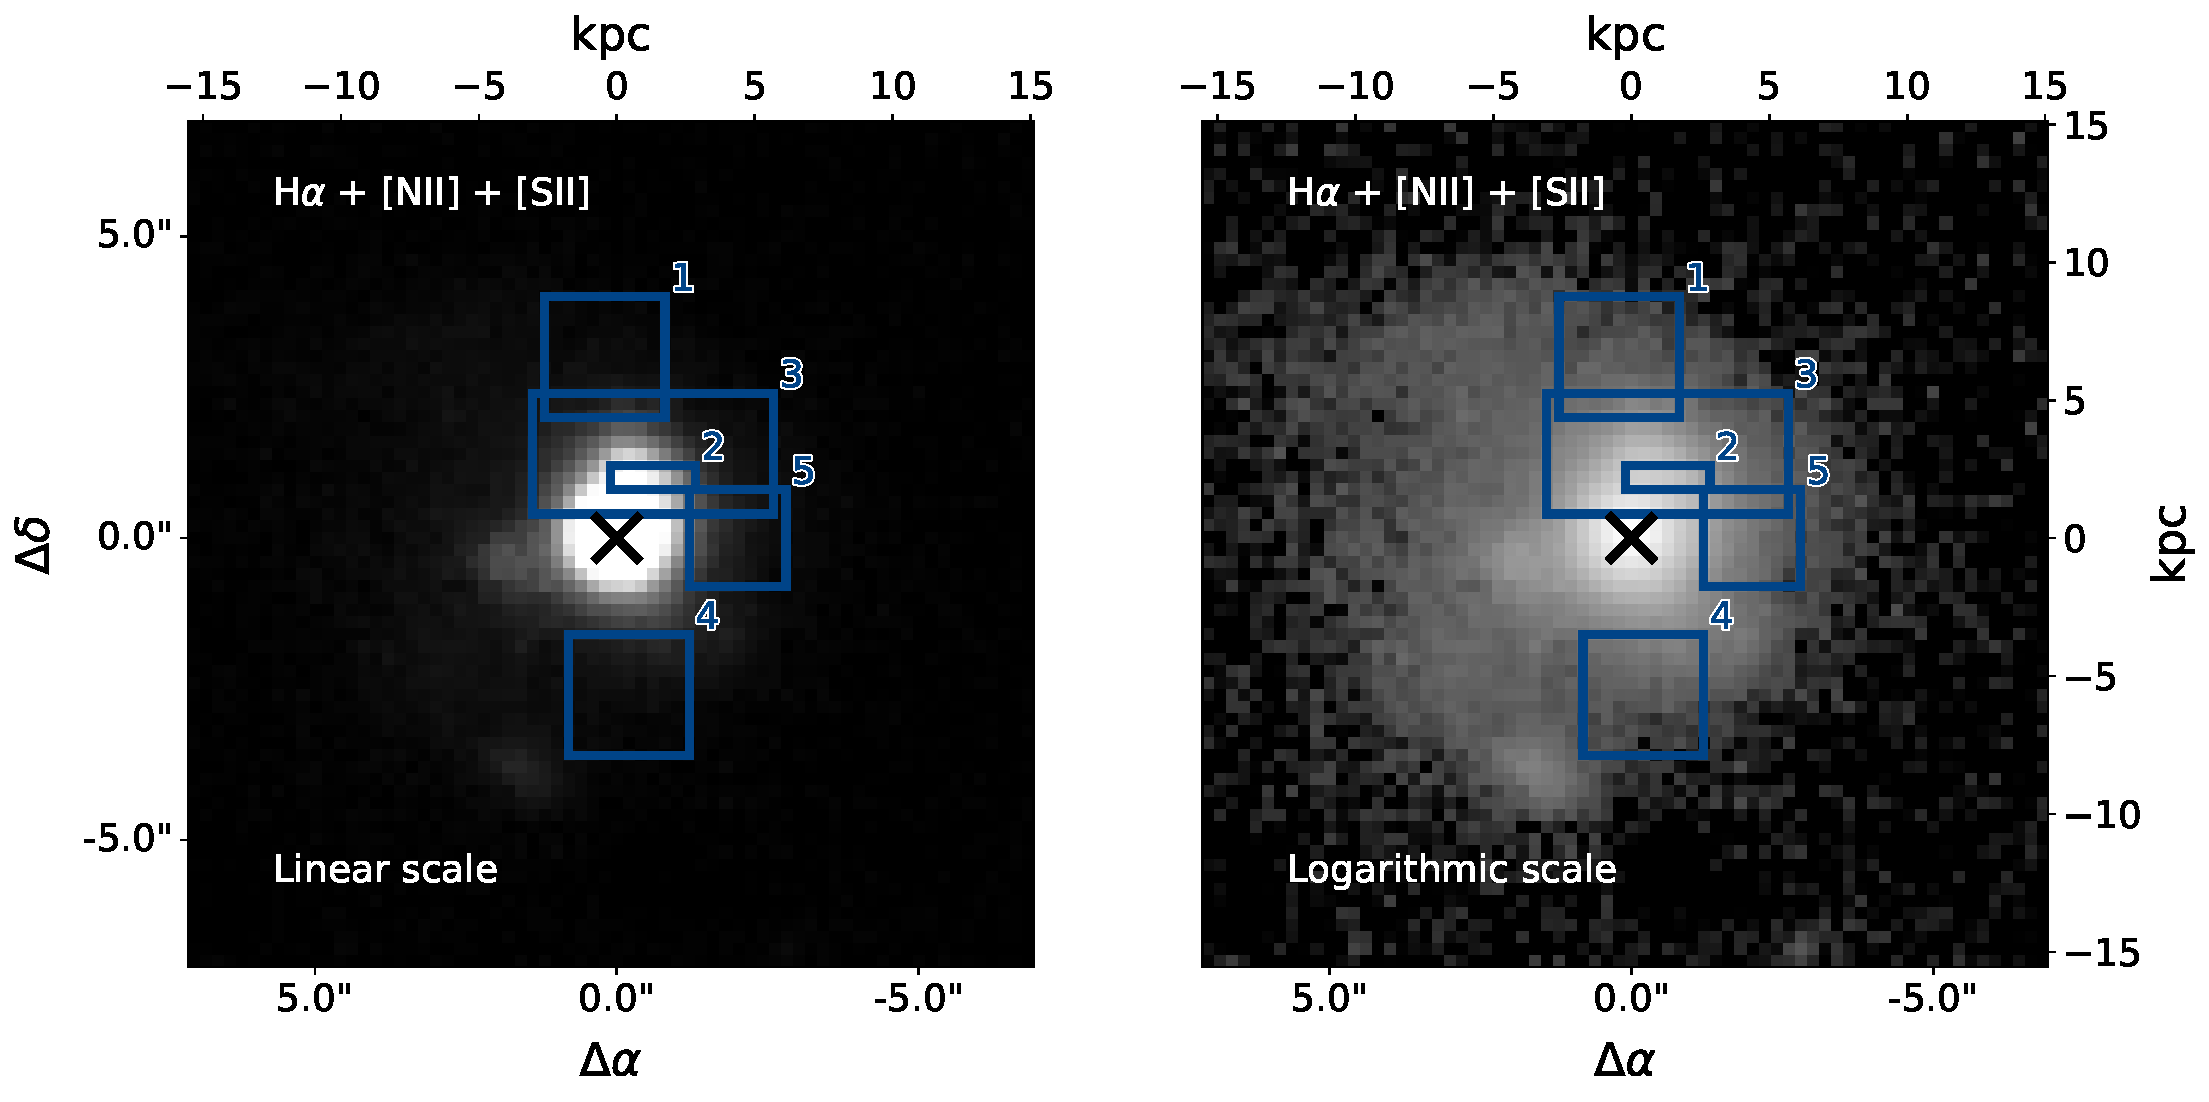
\includegraphics[width=\linewidth, trim={0cm 0 0 0cm}, clip]{figures/muse_f13451_1232/halpha_sii_image_apertures.pdf}
    \caption[Continuum-subtracted H$\alpha$ + {[}NII{]}$\lambda\lambda$6548,6584 + {[}SII{]}$\lambda\lambda$6717,6731 images of F13451+1232, with the locations and sizes of extracted apertures shown.]{Continuum-subtracted H$\alpha$ + [NII]$\lambda\lambda$6548,6584 + [SII]$\lambda\lambda$6717,6731 image (left: linear scale; right: logarithmic scale) of F13451+1232 with the locations and sizes of the selected apertures shown in blue. The aperture numbers are labelled at the top right of each, and the position of the primary nucleus is marked with a black cross.}
    \label{fig: muse_f13451_1232: analysis_and_results: extended_emission: apertures}
\end{figure}

\newpage

\subsubsection{Aperture emission-line fits}
\label{section: muse_f13451_1232: analysis_and_results: extended_emission: aperture_line_fits}

For each aperture, the line profiles of the [OIII]$\lambda\lambda$4959,5007 doublet (used for kinematics), the H$\alpha$ + {[}NII{]}$\lambda\lambda$6548,6584 blend (the former used to determine gas masses), and the {[}SII{]}$\lambda\lambda$6717,6731 doublet (used to determine electron densities) were fit with two methods: one using the nuclear model and $N_\mathrm{g}$ Gaussian components, and the other using only $N_\mathrm{g}$ Gaussian components (free-fitting), mirroring the approach taken earlier. For the nuclear-model fits, in the case of the [OIII]$\lambda\lambda$4959,5007 doublet, the nuclear model described in Section\;\ref{section: muse_f13451_1232: analysis_and_results: seeing: nuclear_aperture_extraction} (Figure\;\ref{fig: muse_f13451_1232: analysis_and_results: seeing: nuclear_aperture_spectrum}; Table\;\ref{tab: muse_f13451_1232: analysis_and_results: seeing: nuclear_model}) was used, while a distinct model for the H$\alpha$ + {[}NII{]}$\lambda\lambda$6548,6584 blend was created using the Bayesian emission line routine with the nuclear aperture. The H$\alpha$ and {[}NII{]}$\lambda\lambda$6548,6584 line profiles were significantly blended, and so the nuclear model consisted of a single Gaussian for each of the lines (with equal line widths, and wavelength separations and [NII] flux ratio taken from atomic physics) and $N_\mathrm{g}$ Gaussian components for the broad blend. For the {[}SII{]}$\lambda\lambda$6717,6731 doublet, the nuclear model was defined using a similar method to that of [OIII]: $N_\mathrm{g}$ Gaussian components were used for each line; constraints from atomic physics \citep{Osterbrock2006} were used to fix the wavelength separation of the lines, and the widths of the lines were set to be equal. However, in this case, the relative peak flux densities of the lines were required to be in the range 0.44\;\textless\;[SII](6717/6731)\;\textless\;1.45.

The emission-line fits produced by both methods (the nuclear model + $N_\mathrm{g}$ Gaussian components, and the free fits) for each aperture are shown in Figure\;\ref{fig: muse_f13451_1232: analysis_and_results: extended_emission: aperture_line_fits}. For each of the diagnostic lines ([OIII], [SII], H$\alpha$ + [NII]), the Bayesian odds of the nuclear-model fits and free fits was used to determine if the nuclear model was required: the more-complex model (i.e. that consisting of the greater number of parameters) was selected if the ratio of its posterior probability to that of the less-complex model was greater than two. The results of this selection for each line blend in each aperture are given in Table\;\ref{tab: muse_f13451_1232: analysis_and_results: extended_emission: aperture_kinematics_energetics}. In the case where the nuclear model was preferred, only the additional (non-nuclear-component) Gaussian components were used to derive gas kinematics and velocities, while in the free-fitting case, all Gaussian components were used.

\clearpage

\begin{figure*}
    \centering
    \caption[Fits to the {[}OIII{]}$\lambda\lambda4959,5007$ doublet, H$\alpha$ + {[}NII{]}$\lambda\lambda$6548,6584 blend, and {[}SII{]}$\lambda\lambda$6717,6731 doublet in apertures extracted from MUSE DEEP data of F13451+1232 using the nuclear model + $N_\mathrm{g}$ Gaussian components and free-fitting approaches.]{Fits to the [OIII]$\lambda\lambda4959,5007$ doublet (top rows), H$\alpha$ + {[}NII{]}$\lambda\lambda$6548,6584 blend (middle rows), and {[}SII{]}$\lambda\lambda$6717,6731 doublet (bottom rows) in the apertures using the nuclear model + $N_\mathrm{g}$ Gaussian components (left column) and free-fitting (right column) approaches. The spectrum extracted from the aperture is shown as a black solid line, the overall fit in each case is shown as a solid red line, the first-order polynomial fit (accounting for the continuum) is shown as a dotted orange line, the components from the nuclear model (left panels only) are shown as a dashed blue line, and the additional Gaussian components (left panels) / free-fit components (right panels) are shown as green dash-dotted lines.\\}
    \label{fig: muse_f13451_1232: analysis_and_results: extended_emission: aperture_line_fits}
    \begin{subfigure}[t]{0.85\linewidth}
        \begin{minipage}{0.48\linewidth}
            \centering
            \textbf{Nuclear-model fits}
        \end{minipage}
        \hfill
        \begin{minipage}{0.42\linewidth}
            \centering
            \textbf{Free fits}
        \end{minipage}
        \vfill
        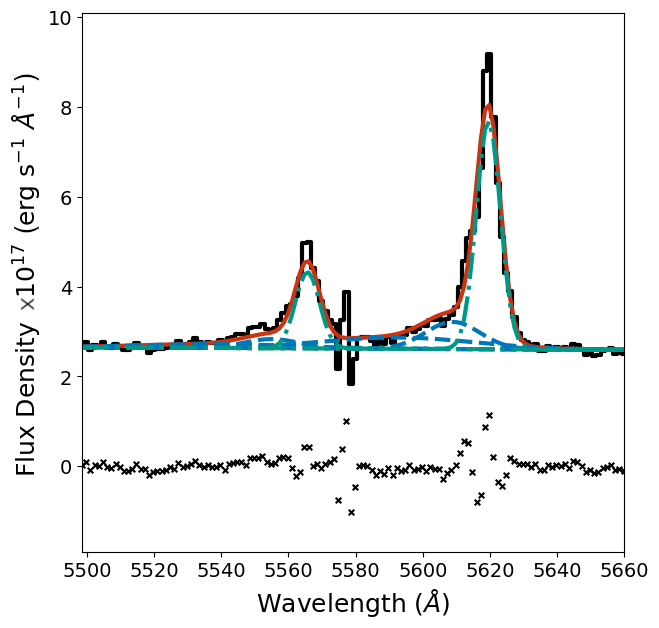
\includegraphics[width=0.45\textwidth]{figures/muse_f13451_1232/line_fits/ap1_oiii.png}
        \hfill
        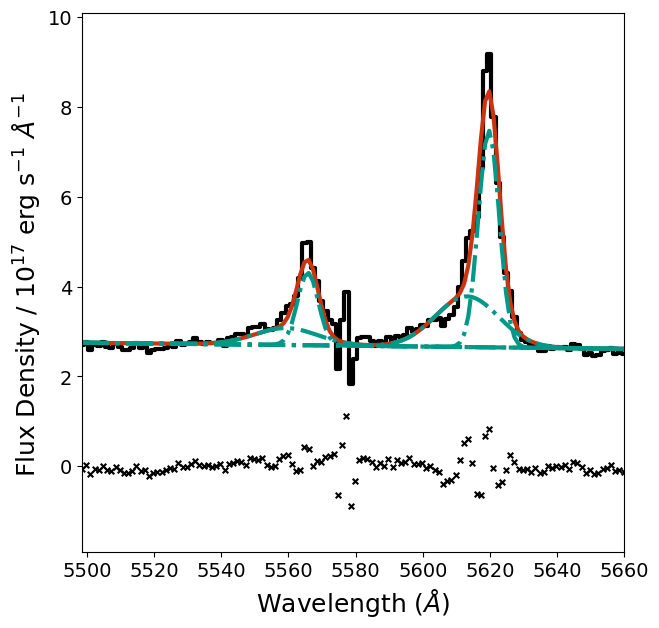
\includegraphics[width=0.45\textwidth]{figures/muse_f13451_1232/line_fits/ap1_oiii_no_nuclear_model.png}
        \vfill
        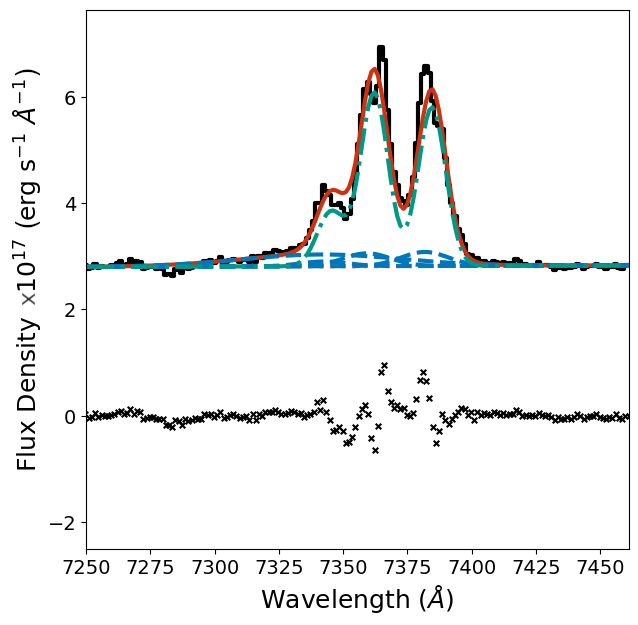
\includegraphics[width=0.435\textwidth]{figures/muse_f13451_1232/line_fits/ap1_halpha.png}
        \hspace{1.42cm}
        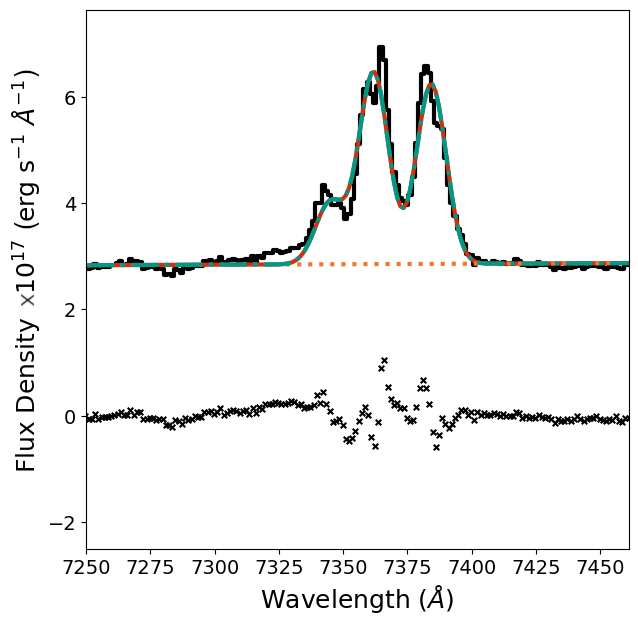
\includegraphics[width=0.435\textwidth]{figures/muse_f13451_1232/line_fits/ap1_halpha_no_nuclear_model.png}
        \vfill
        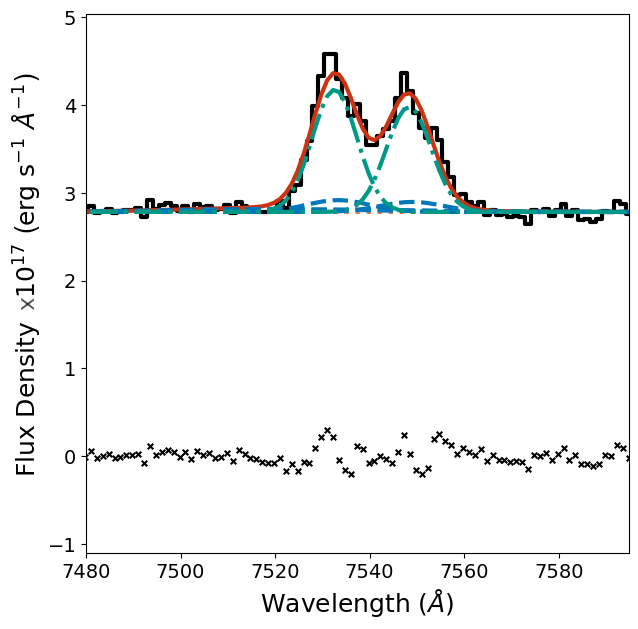
\includegraphics[width=0.45\textwidth]{figures/muse_f13451_1232/line_fits/ap1_sii.png}
        \hspace{1.3cm}
        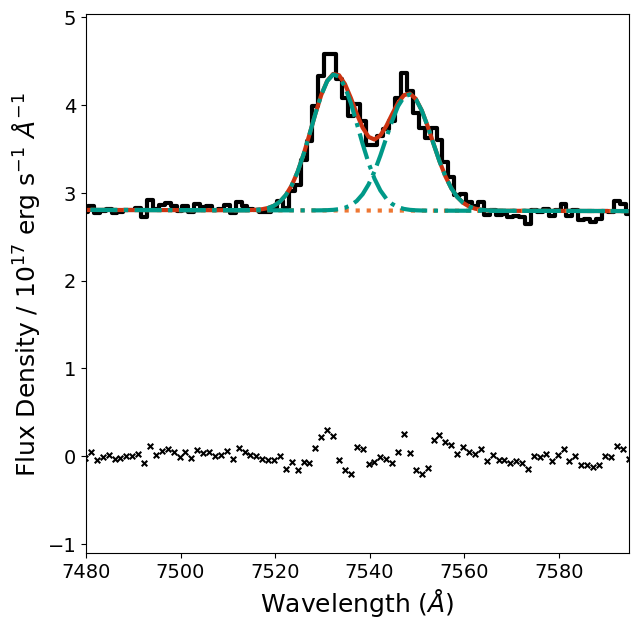
\includegraphics[width=0.45\textwidth]{figures/muse_f13451_1232/line_fits/ap1_sii_no_nuclear_model.png}
        \label{fig: muse_f13451_1232: analysis_and_results: extended_emission: ap1_line_fits}
        \caption{The line fits for the spectrum extracted from Aperture 1. The feature at $\sim$5580\;{\AA} is instrumental, and did not have a significant impact on the resulting fits. }
    \end{subfigure}
\end{figure*}
\begin{figure*}\ContinuedFloat
    \centering
    \begin{subfigure}[t]{0.9\linewidth}
        \begin{minipage}{0.48\linewidth}
            \centering
            \textbf{Nuclear-model fits}
        \end{minipage}
        \hfill
        \begin{minipage}{0.42\linewidth}
            \centering
            \textbf{Free fits}
        \end{minipage}
        \vfill
        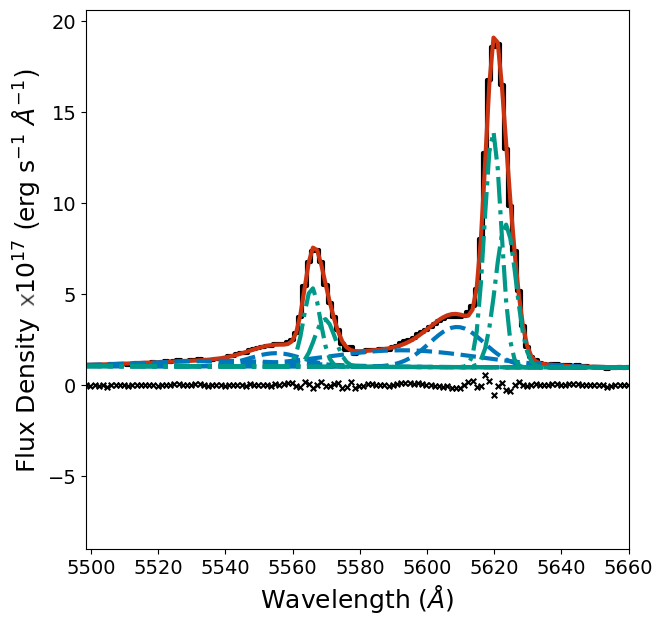
\includegraphics[width=0.45\textwidth]{figures/muse_f13451_1232/line_fits/ap2_oiii.png}
        \hfill
        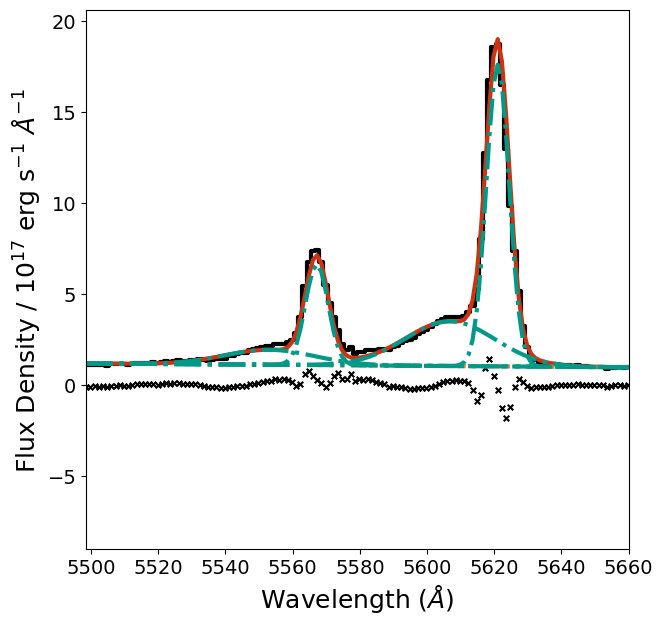
\includegraphics[width=0.45\textwidth]{figures/muse_f13451_1232/line_fits/ap2_oiii_no_nuclear_model.png}
        \vfill
        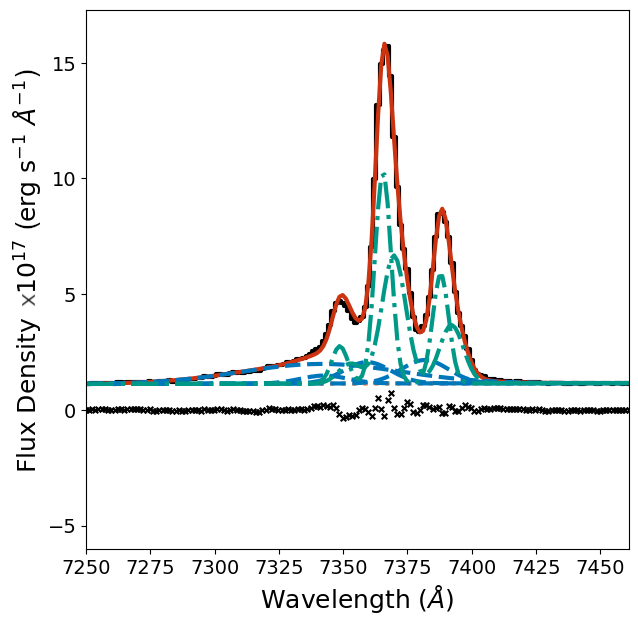
\includegraphics[width=0.435\textwidth]{figures/muse_f13451_1232/line_fits/ap2_halpha.png}
        \hspace{1.42cm}
        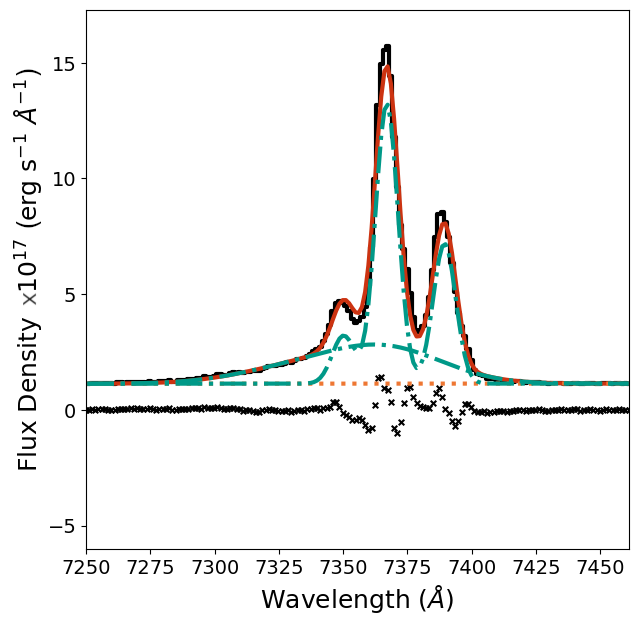
\includegraphics[width=0.435\textwidth]{figures/muse_f13451_1232/line_fits/ap2_halpha_no_nuclear_model.png}
        \vfill
        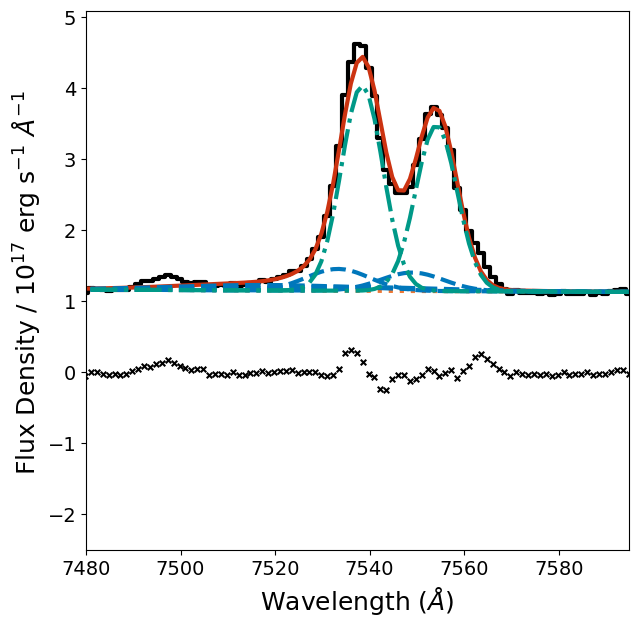
\includegraphics[width=0.45\textwidth]{figures/muse_f13451_1232/line_fits/ap2_sii.png}
        \hspace{1.3cm}
        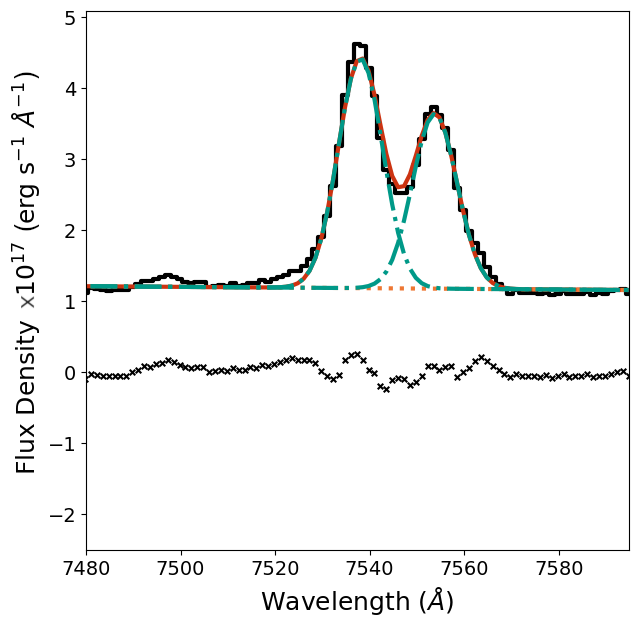
\includegraphics[width=0.45\textwidth]{figures/muse_f13451_1232/line_fits/ap2_sii_no_nuclear_model.png}
        \label{fig: muse_f13451_1232: analysis_and_results: extended_emission: ap2_line_fits}
        \caption{The line fits for the spectrum extracted from Aperture 2.}
    \end{subfigure}
\end{figure*}
\begin{figure*}\ContinuedFloat
    \centering
    \begin{subfigure}[t]{0.9\linewidth}
        \begin{minipage}{0.48\linewidth}
            \centering
            \textbf{Nuclear-model fits}
        \end{minipage}
        \hfill
        \begin{minipage}{0.42\linewidth}
            \centering
            \textbf{Free fits}
        \end{minipage}
        \vfill
        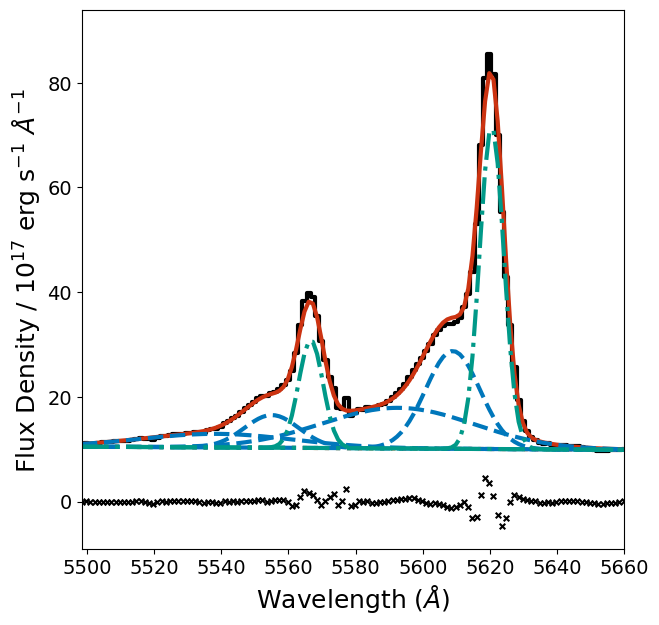
\includegraphics[width=0.45\textwidth]{figures/muse_f13451_1232/line_fits/ap3_oiii.png}
        \hfill
        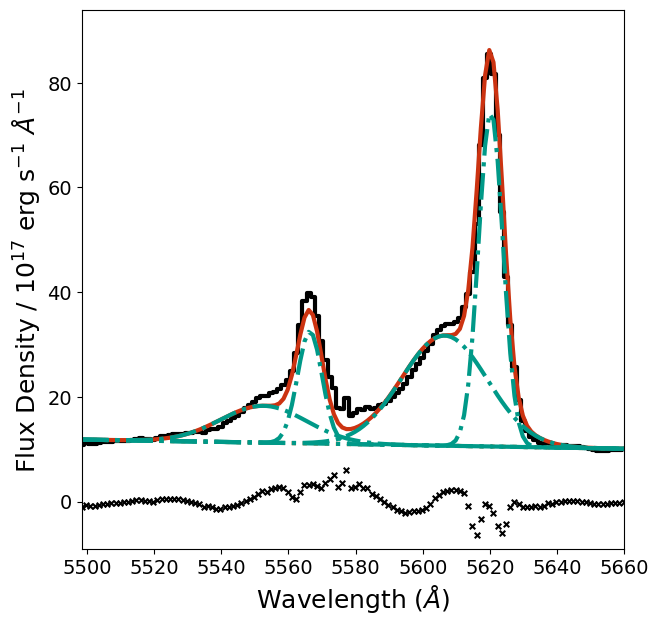
\includegraphics[width=0.45\textwidth]{figures/muse_f13451_1232/line_fits/ap3_oiii_no_nuclear_model.png}
        \vfill
        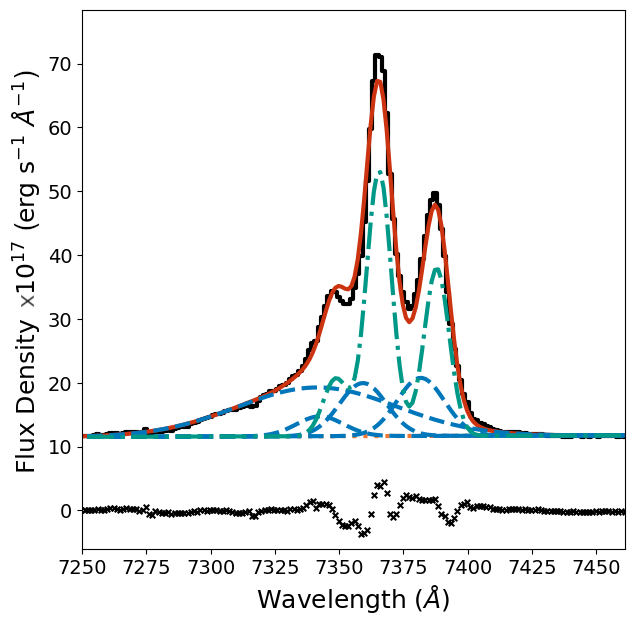
\includegraphics[width=0.435\textwidth]{figures/muse_f13451_1232/line_fits/ap3_halpha.png}
        \hspace{1.42cm}
        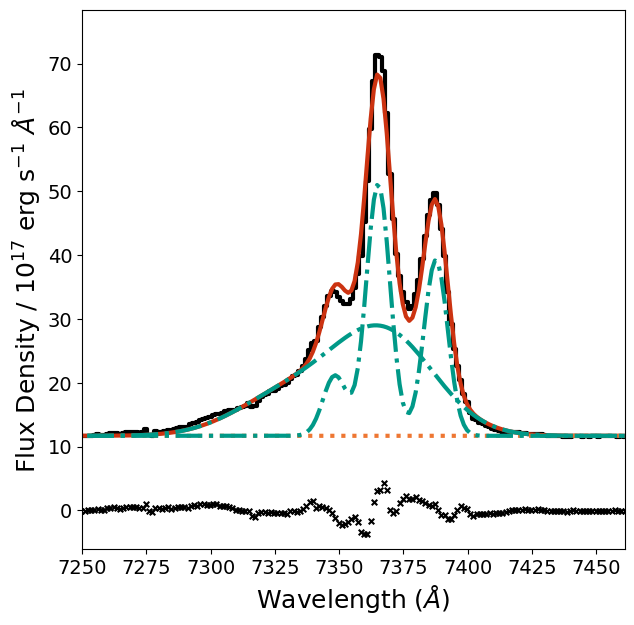
\includegraphics[width=0.435\textwidth]{figures/muse_f13451_1232/line_fits/ap3_halpha_no_nuclear_model.png}
        \vfill
        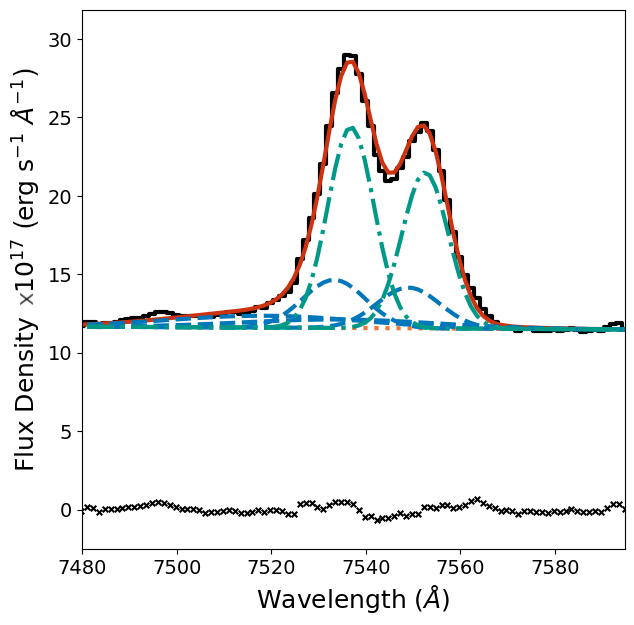
\includegraphics[width=0.45\textwidth]{figures/muse_f13451_1232/line_fits/ap3_sii.png}
        \hspace{1.3cm}
        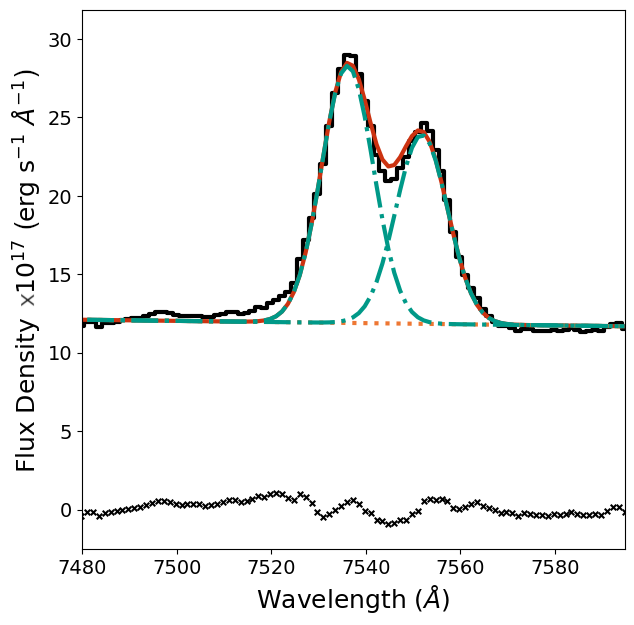
\includegraphics[width=0.45\textwidth]{figures/muse_f13451_1232/line_fits/ap3_sii_no_nuclear_model.png}
        \label{fig: muse_f13451_1232: analysis_and_results: extended_emission: ap3_line_fits}
        \caption{The line fits for the spectrum extracted from Aperture 3.}
    \end{subfigure}
\end{figure*}
\begin{figure*}\ContinuedFloat
    \centering
    \begin{subfigure}[t]{0.9\linewidth}
        \begin{minipage}{0.48\linewidth}
            \centering
            \textbf{Nuclear-model fits}
        \end{minipage}
        \hfill
        \begin{minipage}{0.42\linewidth}
            \centering
            \textbf{Free fits}
        \end{minipage}
        \vfill
        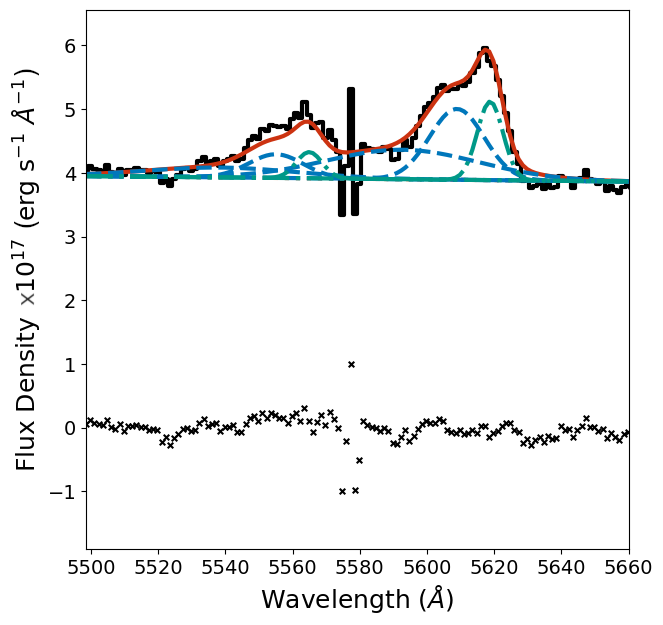
\includegraphics[width=0.45\textwidth]{figures/muse_f13451_1232/line_fits/ap4_oiii.png}
        \hfill
        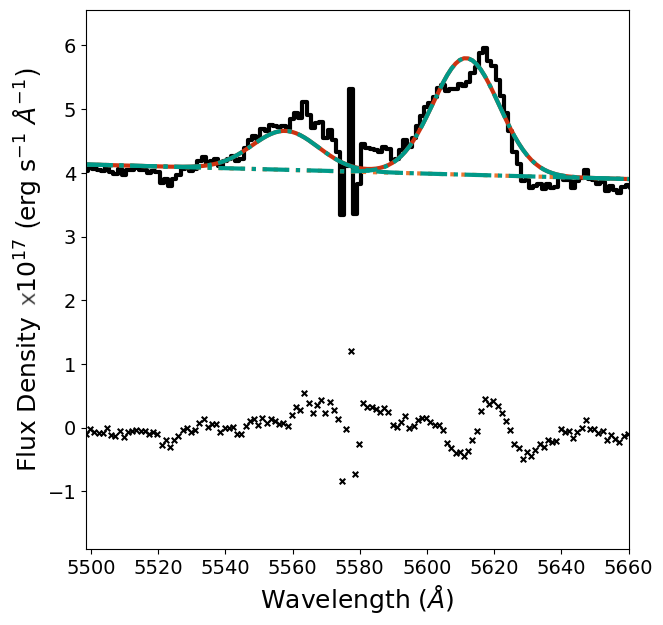
\includegraphics[width=0.45\textwidth]{figures/muse_f13451_1232/line_fits/ap4_oiii_no_nuclear_model.png}
        \vfill
        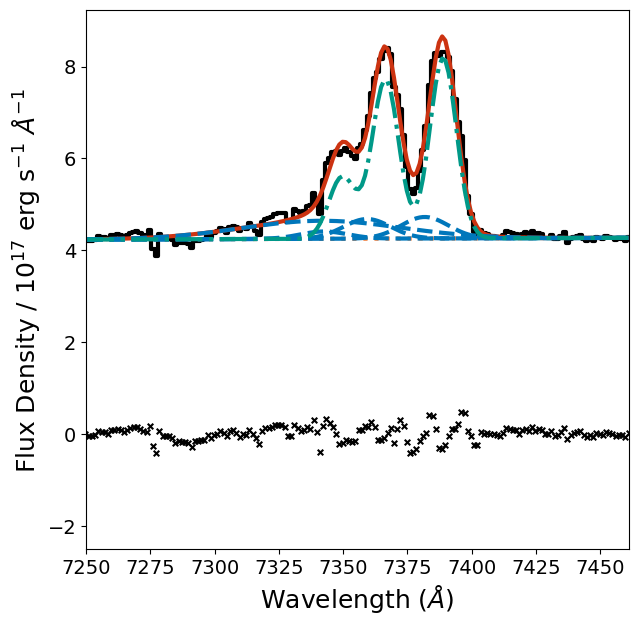
\includegraphics[width=0.435\textwidth]{figures/muse_f13451_1232/line_fits/ap4_halpha.png}
        \hspace{1.42cm}
        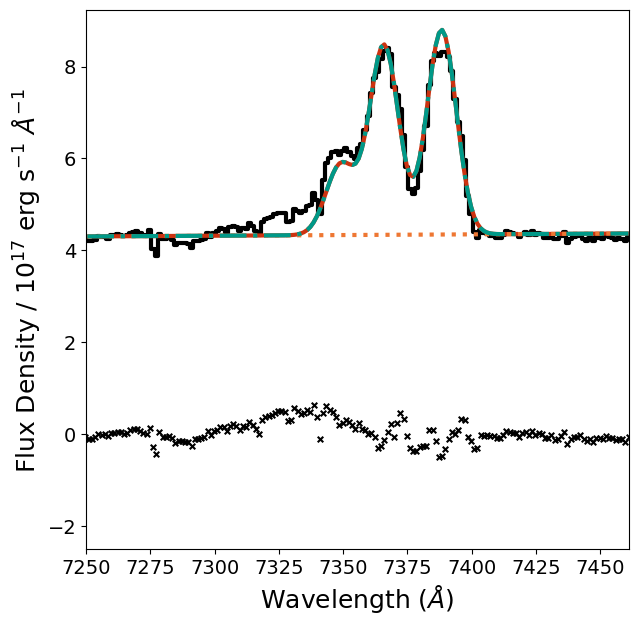
\includegraphics[width=0.435\textwidth]{figures/muse_f13451_1232/line_fits/ap4_halpha_no_nuclear_model.png}
        \vfill
        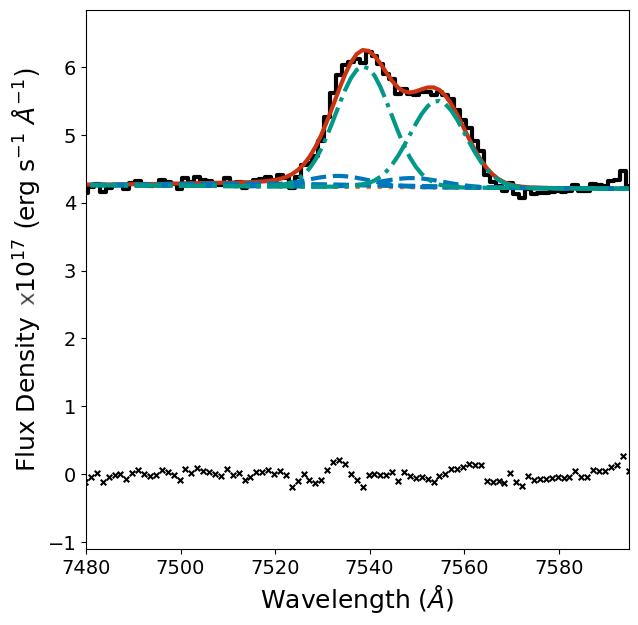
\includegraphics[width=0.45\textwidth]{figures/muse_f13451_1232/line_fits/ap4_sii.png}
        \hspace{1.3cm}
        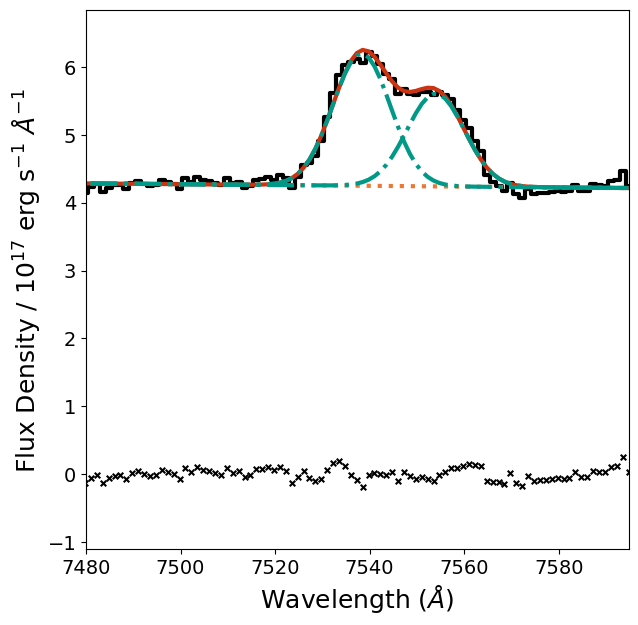
\includegraphics[width=0.45\textwidth]{figures/muse_f13451_1232/line_fits/ap4_sii_no_nuclear_model.png}
        \label{fig: muse_f13451_1232: analysis_and_results: extended_emission: ap4_line_fits}
        \caption{The line fits for the spectrum extracted from Aperture 4.}
    \end{subfigure}
\end{figure*}
\begin{figure*}\ContinuedFloat
    \centering
    \begin{subfigure}[t]{0.9\linewidth}
        \begin{minipage}{0.48\linewidth}
            \centering
            \textbf{Nuclear-model fits}
        \end{minipage}
        \hfill
        \begin{minipage}{0.42\linewidth}
            \centering
            \textbf{Free fits}
        \end{minipage}
        \vfill
        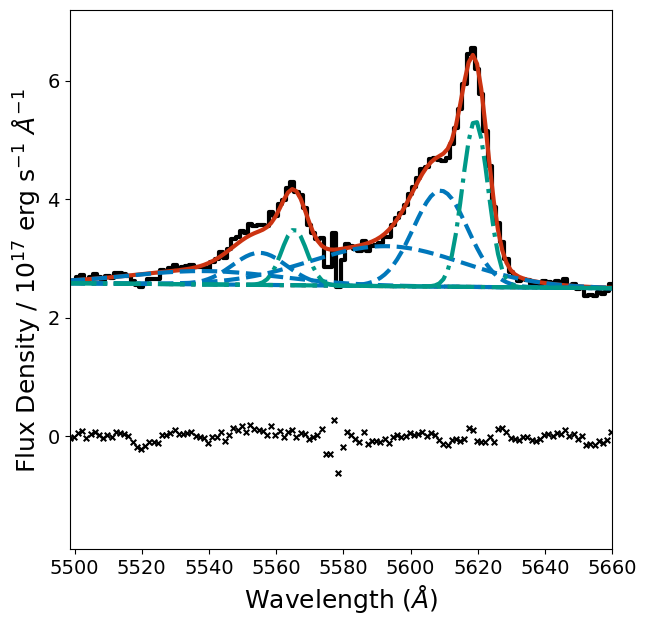
\includegraphics[width=0.45\textwidth]{figures/muse_f13451_1232/line_fits/ap5_oiii.png}
        \hfill
        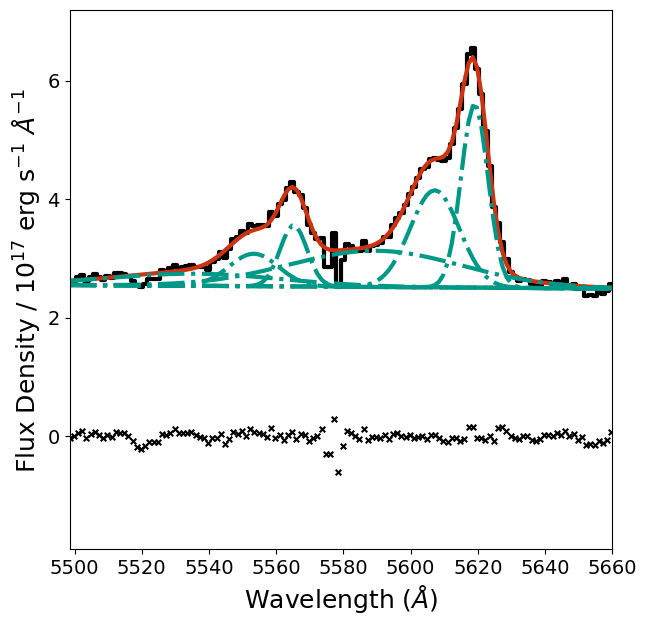
\includegraphics[width=0.45\textwidth]{figures/muse_f13451_1232/line_fits/ap5_oiii_no_nuclear_model.png}
        \vfill
        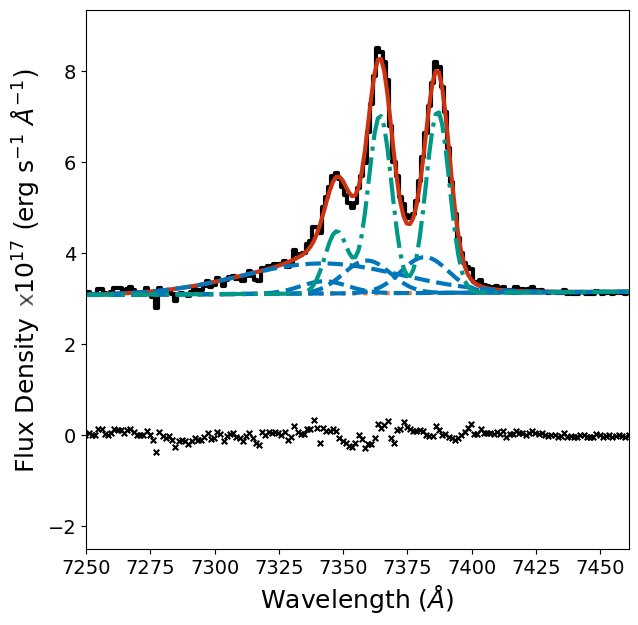
\includegraphics[width=0.435\textwidth]{figures/muse_f13451_1232/line_fits/ap5_halpha.png}
        \hspace{1.42cm}
        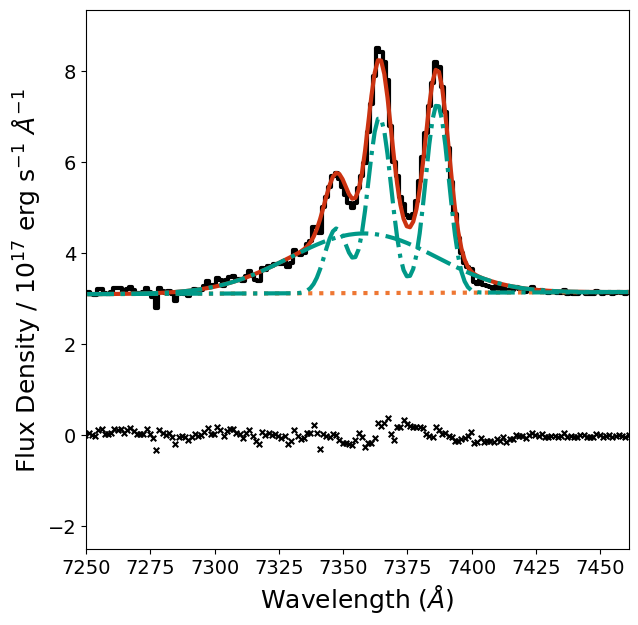
\includegraphics[width=0.435\textwidth]{figures/muse_f13451_1232/line_fits/ap5_halpha_no_nuclear_model.png}
        \vfill
        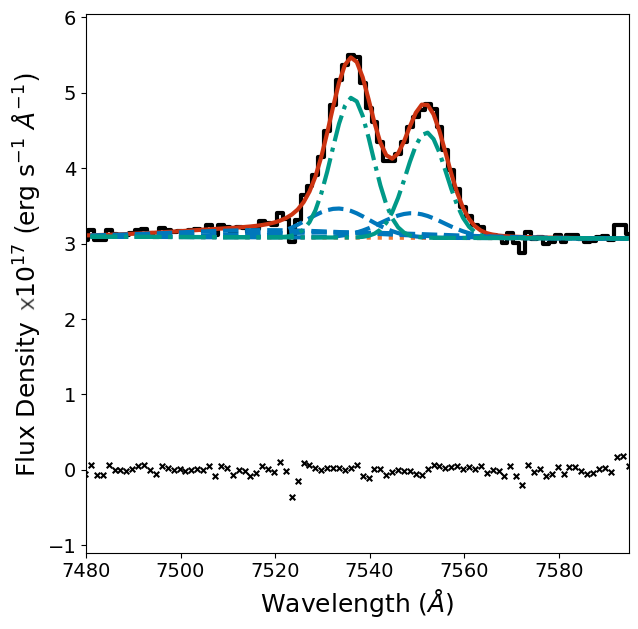
\includegraphics[width=0.45\textwidth]{figures/muse_f13451_1232/line_fits/ap5_sii.png}
        \hspace{1.3cm}
        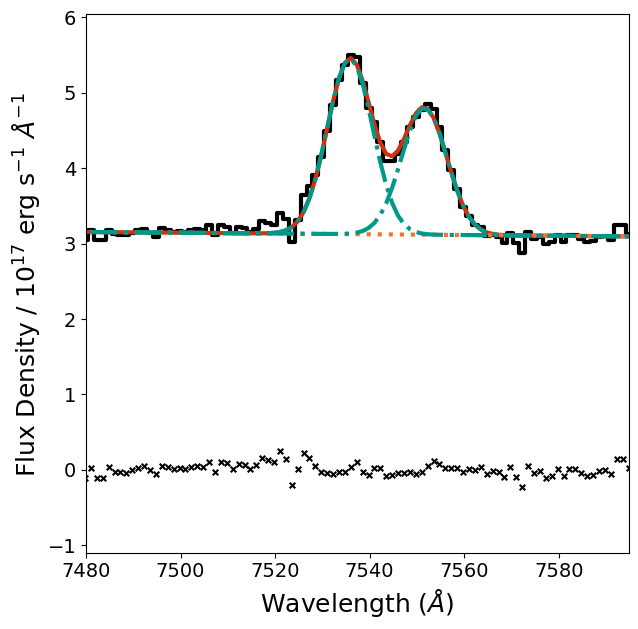
\includegraphics[width=0.45\textwidth]{figures/muse_f13451_1232/line_fits/ap5_sii_no_nuclear_model.png}
        \label{fig: muse_f13451_1232: analysis_and_results: extended_emission: ap5_line_fits}
        \caption{The line fits for the spectrum extracted from Aperture 5.}
    \end{subfigure}
\end{figure*}

\clearpage
\newpage

\subsubsection{Kinematics, physical conditions, and energetics of the extended emission}
\label{section: muse_f13451_1232: analysis_and_results: extended_emission: aperture_properties}
\vspace*{-6pt}
In order to place upper limits on the energetics of any real, spatially-extended warm-ionised outflows, the masses, mass outflow rates, and kinetic powers of the warm-ionised gas in each aperture were calculated under the assumption that it is outflowing. As discussed and demonstrated in Chapters \ref{chapter: introduction}, \ref{chapter: xshooter_ic5063}, and \ref{chapter: stis_seyferts}, a major source of uncertainty in deriving warm-ionised outflow kinetic powers is the electron density; proper measurement requires robust diagnostics that are sensitive to a range of values and insensitive to emission-line blending effects, such as the transauroral-line technique \citep{Holt2011}. Since the required transauroral lines of [SII] and [OII] are not contained in the spectral coverage of MUSE, here the electron density for each aperture was determined using the traditional [SII](6717/6731) ratio with strict measurement criteria, as was previously done for VLT/Xshooter spectra of the Sey\;2 galaxy IC\;5063 in Section\;\ref{section: xshooter_ic5063: properties_of_outflowing_gas: uvb_vis_analysis_and_results: trad_densities}: if a measured ratio was not 3$\sigma$ away from the theoretical lower or upper ratio limit (\mbox{0.30\;\textless\;[SII](6717/6731)\;\textless\;1.45}), then a $3\sigma$ limit was taken in the opposite direction (to give an upper or lower limit). In this way, it was ensured that the measured densities were accurate, and not subject to effects resulting from the ratio saturating at high or low values. The measured [SII] ratios (or upper/lower limits) were then used to determine electron densities using the \textsc{PyNeb Python} module. Due to the necessary lines (namely [OIII]$\lambda4363$) not being well detected in the apertures, it was not possible to measure electron temperatures for the extended gas. Therefore, a temperature of $T_e=10,000$\;K (typical for the warm ionised phase: Chapters \ref{chapter: xshooter_ic5063} and \ref{chapter: stis_seyferts}) was assumed in the electron density calculations.

Next, the flux of the H$\alpha$ line was determined by measuring the total flux of all Gaussian components that corresponded to the H$\alpha$ line in the fitted blends (i.e. not the nuclear-model components). Note that the H$\beta$ line itself was not measured due to its significantly lower flux compared to H$\alpha$, resulting in it not being well detected in the majority of the apertures. To estimate the H$\beta$ flux --- required to estimate gas masses --- the emissivity ratio $j_\mathrm{H\alpha}/j_\mathrm{H\beta}=2.863$ at $T_e=10,000$\;K and $n_e=10^2$\;cm$^{-3}$ \citep{Osterbrock2006} was used. Warm-ionised gas masses for each aperture were then calculated using the derived H$\beta$ luminosities with Equation \ref{eq: introduction: outflows: energetics: mout}, taking $\alpha^\mathrm{eff}_\mathrm{H\beta}=3.02\times10^{-14}$\;cm$^{-3}$\;s$^{-1}$ (for $T_e=10,000$\;K and $n_e=10^2$\;cm$^{-3}$) and the derived electron density for the aperture.

The gas kinematics in each aperture were determined using the [OIII]$\lambda\lambda4959,5007$ doublet in two ways, following the methodology outlined in Section\;\ref{section: xshooter_ic5063: properties_of_outflowing_gas: uvb_vis_analysis_and_results: kinematics} (see also \citealt{Rose2018}). Flux-weighted velocity shifts ($v_\mathrm{w}$) and FWHMs (FWHM$_\mathrm{w}$) were determined using Equations \ref{eq: xshooter_ic5063: flux_velocity} and \ref{eq: xshooter_ic5063: flux_width}, respectively; the flux-weighted FWHMs were corrected for instrumental broadening by subtracting the instrumental width of MUSE from the width of each constituent Gaussian component in quadrature. 10th and 90th percentile velocity shifts ($v_\mathrm{10}$ and $v_\mathrm{90}$: the velocity containing 10 and 90\;per\;cent of the total emission-line-component flux, respectively) were also determined and used to produce the non-parametric $W_\mathrm{80}$ velocity width for each aperture. The resulting kinematics are given in Tables \ref{tab: muse_f13451_1232: analysis_and_results: extended_emission: aperture_kinematics_energetics} and \ref{tab: muse_f13451_1232: analysis_and_results: extended_emission: aperture_kinematics_energetics_free}. The percentile velocity shifts were subsequently used with Equation \ref{eq: introduction: outflows: energetics: mout_rate} to produce mass outflow rates, assuming $A=1$ (see Section\;\ref{section: introduction: outflows: energetics}) and taking the outflow radius (${\Delta}R$) to be the radial extent of the given aperture in the direction from the nucleus. Finally, kinetic powers were determined using Equation\;\ref{eq: introduction: outflows: energetics: ekin} with the estimated mass flow rates and the percentile velocities (and assuming no velocity width; i.e. $\sigma=0$\;km\;s$^{-1}$) --- percentile velocities were used because any potential outflowing gas in the apertures would not be spatially-resolved (see discussion in Section \ref{section: introduction: outflows: kinematics_and_geometry: kinematics}), and in this way, any real outflow kinematics will not be underestimates. Coupling efficiencies for each aperture were estimated by comparing the measured kinetic powers to the AGN bolometric luminosity of F13451+1232 ($L_\mathrm{bol}=4.8\times10^{45}$\;erg\;s$^{-1}$: \citealt{Rose2018}). The resulting gas properties for each aperture are presented in Tables \ref{tab: muse_f13451_1232: analysis_and_results: extended_emission: aperture_kinematics_energetics} and \ref{tab: muse_f13451_1232: analysis_and_results: extended_emission: aperture_kinematics_energetics_free}.

For the beam-smearing-corrected case (in which the nuclear model was used in the fits to the extended emission; Table\;\ref{tab: muse_f13451_1232: analysis_and_results: extended_emission: aperture_kinematics_energetics}), the kinematics are modest (50\;\textless\;$v_w$\;\textless\;180\;km\;s$^{-1}$; 370\;\textless\;$v_p$\;\textless\;440\;km\;s$^{-1}$; 300\;\textless\;FWHM$_w$\;\textless\;470\;km\;s$^{-1}$; 400\;\textless\;$W_\mathrm{80}$\;\textless\;470\;km\;s$^{-1}$). Similarly, the mass outflow rates and kinetic powers --- despite being lower limits for apertures 2 and 4 --- are also low (0.14\;\textless\;$\dot{M}_\mathrm{out}$\;\textless\;$1.50$\;M$_\odot$\;yr$^{-1}$; $1.21\times10^{-4}$\;\textless\;$\dot{E}_\mathrm{kin}$\;\textless\;$1.88\times10^{-3}$\;per\;cent of $L_\mathrm{bol}$). For all apertures, the inclusion of the nuclear model in the fits to the extended emission produced statistically-better fits to the [OIII] emission lines, further demonstrating that beam-smeared nuclear-outflow emission contributes significant flux up to radial distances of $r\sim4$\;arcseconds ($r\sim9$\;kpc; i.e. the maximum radial distance of the apertures from the primary nucleus). Furthermore, when beam smearing is not accounted for --- demonstrated here by the free-fitting case (Table\;\ref{tab: muse_f13451_1232: analysis_and_results: extended_emission: aperture_kinematics_energetics_free}) --- the derived mass outflow rates are significantly higher (up to $\dot{M}_\mathrm{out}=7.4\pm4.8$\;M$_\odot$\;yr$^{-1}$). However, even in this case, the mass outflow rates are much lower than that of the total nuclear outflow in F13451+1232 ($\dot{M}_\mathrm{out}\sim230$\;M$_\odot$\;yr$^{-1}$: Chapter\;\ref{chapter: alma_f13451_1232}), and the maximum measured kinetic power (Aperture\;3: $\dot{E}_\mathrm{kin}=0.06\pm0.02$\;per\;cent of $L_\mathrm{bol}$) is far below the range of values required by models of galaxy evolution (\textgreater\;0.15\;per\;cent of $L_\mathrm{bol}$: e.g. \citealt{Springel2005, Hopkins2010, Schaye2015, Dubois2016}).

Finally, I highlight that the mass outflow rates, kinetic powers, and coupling efficiencies presented here are likely to represent upper limits for any real, spatially-extended outflows, as it is assumed (but not established) that the additional non-nuclear components represent outflowing gas, although their kinematics are not consistent with this scenario.

\clearpage

\begin{table}
    \begin{subtable}{\textwidth}
        \renewcommand{\arraystretch}{1.2}
        \centering
        \centerline{
        \begin{tabular}{ccccccc}
            \multirow{2}{*}{Aperture} & Nuclear model & $v_w$ & FWHM$_w$ & $v_p$ & $W_\mathrm{80}$ & EW$_\mathrm{H\alpha}$ \\
                &   required    & (km\;s$^{-1}$) & (km\;s$^{-1}$) & (km\;s$^{-1}$) & (km\;s$^{-1}$) & ({\AA}) \\
            \hline \\
            \multirow{3}{*}{1} & [OIII] &   \multirow{3}{*}{$88\pm2$} &   \multirow{3}{*}{$427\pm16$}   &   \multirow{3}{*}{$370\pm10$}   &   \multirow{3}{*}{$401\pm10$} & \multirow{3}{*}{$-19.5\pm1.2$}  \\
                &   --- &   &   &   &   \\
                &   --- &   &   &   &   \\
                &   &   &   &   &   \\
            \multirow{3}{*}{2} & [OIII] &   \multirow{3}{*}{$179\pm96$} &   \multirow{3}{*}{$311\pm191$}   &   \multirow{3}{*}{$437\pm174$}   &   \multirow{3}{*}{$401\pm175$} & \multirow{3}{*}{$-113.1\pm28.8$}  \\
                &   H$\alpha$ &   &   &   &   \\
                &   --- &   &   &   &   \\
                &   &   &   &   &   \\
            \multirow{3}{*}{3} & [OIII] &   \multirow{3}{*}{$141\pm1$} &   \multirow{3}{*}{$432\pm5$}   &   \multirow{3}{*}{$437\pm4$}   &   \multirow{3}{*}{$467\pm4$} & \multirow{3}{*}{$-40.8\pm3.7$}   \\
                &   --- &   &   &   &   \\
                &   [SII] &   &   &   &   \\
                &   &   &   &   &   \\
            \multirow{3}{*}{4} & [OIII] &   \multirow{3}{*}{$51\pm4$} &   \multirow{3}{*}{$460\pm49$}   &   \multirow{3}{*}{$370\pm17$}   &   \multirow{3}{*}{$467\pm27$} & \multirow{3}{*}{$-14.4\pm1.2$}   \\
                &   --- &   &   &   &   \\
                &   --- &   &   &   &   \\
                &   &   &   &   &   \\
            \multirow{3}{*}{5} & [OIII] &   \multirow{3}{*}{$73\pm3$} &   \multirow{3}{*}{$467\pm15$}   &   \multirow{3}{*}{$370\pm14$}   &   \multirow{3}{*}{$467\pm15$} & \multirow{3}{*}{$-11.1\pm0.9$}   \\
                &   H$\alpha$ &   &   &   &   \\
                &   --- &   &   &   &   \\
                &   &   &   &   &   \\
        \end{tabular}
        }
    \end{subtable} \\
    \begin{subtable}{\textwidth}
        \renewcommand{\arraystretch}{1.2}
        \centering
        \begin{tabular}{cccccc}
            \multirow{2}{*}{Aperture} & \multirow{2}{*}{log$_{10}$($n_e$[cm$^{-3}$])} & $M$ ($\times10^6$  & $\dot{M}$ & $\dot{E}_\mathrm{kin}$ ($\times10^{40}$& $\epsilon_f$ ($\times10^{-4}$ \\
                &      & M$_\odot$) & (M$_\odot$\;yr$^{-1}$) &  erg\;s$^{-1}$) & per\;cent) \\
            \hline \\
            1   & $2.53^{+0.34}_{-0.64}$ & $1.57\pm0.42$ & $0.14\pm0.04$ & $0.58\pm0.16$ & $1.21\pm0.33$  \\
            2   & \textless\;2.53 & \textgreater\;$4.10$ & \textgreater\;0.94 & \textgreater\;$4.07$ & \textgreater\;$8.48$   \\
            3   & $2.24^{+0.36}_{-0.62}$ & $29.5\pm8.3$ & $1.50\pm0.42$ & $9.04\pm0.91$ & $18.8\pm3.5$   \\
            4   & \textless\;$2.41$ & \textgreater\;$2.34$ & \textgreater\;0.20 & \textgreater\;$0.87$ & \textgreater\;$1.81$ \\
            5   & \textless\;$2.42$ & \textgreater\;$1.74$ & \textgreater\;0.15 & \textgreater\;$0.65$ & \textgreater\;$1.35$ \\
        \end{tabular} \\
    \end{subtable} \\
    \vspace{0.2cm} \\
    \caption[Beam-smearing-corrected {[}OIII{]} kinematics (flux weighted velocity shift, intrinsic flux-weighted FWHM, percentile velocity, and non-parametric velocity width $W_\mathrm{80}$), electron densities, masses, flow rates, kinetic powers, and coupling efficiencies for the apertures extracted from the MUSE-DEEP datacube of F13451+1232.]{Beam-smearing-corrected [OIII] kinematics (flux weighted velocity shift, intrinsic flux-weighted FWHM, percentile velocity, and non-parametric velocity width $W_\mathrm{80}$), electron densities, masses, flow rates, kinetic powers, and coupling efficiencies for the apertures extracted from the MUSE-DEEP datacube (Figure\;\ref{fig: muse_f13451_1232: analysis_and_results: extended_emission: apertures}). The `Nuclear model required' column indicates if including the nuclear models (e.g. Figure\;\ref{fig: muse_f13451_1232: analysis_and_results: seeing: nuclear_aperture_spectrum}) in the modelling of the [OIII]$\lambda\lambda4959,5007$, H$\alpha$ + [NII], and [SII]$\lambda\lambda6717,6731$ line profiles produced better fits --- if so, only the additional (non-nuclear-model) Gaussian components were used to derive gas properties. Equivalent widths (EW) for the H$\alpha$ line are also given.}
    \label{tab: muse_f13451_1232: analysis_and_results: extended_emission: aperture_kinematics_energetics}
\end{table}

\newpage

\vfill

\begin{table}
    \begin{subtable}{\textwidth}
        \centering
        \renewcommand{\arraystretch}{1.2}
        \begin{tabular}{cccccc}
            \multirow{2}{*}{Aperture} & $v_w$ & FWHM$_w$ & $v_p$ & $W_\mathrm{80}$ \\
                    & (km\;s$^{-1}$) & (km\;s$^{-1}$) & (km\;s$^{-1}$) & (km\;s$^{-1}$) \\
            \hline \\
            1 & $-48\pm9$ & $695\pm158$ & $-498\pm93$ & $868\pm116$ \\
            2 & $-109\pm3$ & $868\pm31$ & $-898\pm19$ & $1335\pm21$ \\
            3 & $-266\pm4$ & $1057\pm21$ & $-1099\pm13$ & $1469\pm14$ \\
            4 & $-331\pm10$ & $1226\pm54$ & $-898\pm26$ & $1268\pm28$ \\
            5 & $-740\pm119$ & $1683\pm437$ & $-2300\pm249$ & $2600\pm250$ \\
        \end{tabular}
    \end{subtable} \\
    \vspace*{1cm} \\
    \begin{subtable}{\textwidth}
        \centering
        \renewcommand{\arraystretch}{1.2}
        \begin{tabular}{cccccc}
            \multirow{2}{*}{Aperture} & \multirow{2}{*}{log$_{10}$($n_e$[cm$^{-3}$])} & $M$ ($\times10^6$  & $\dot{M}$ & $\dot{E}_\mathrm{kin}$ ($\times10^{40}$& $\epsilon_f$ ($\times10^{-4}$ \\
                &      & M$_\odot$) & (M$_\odot$\;yr$^{-1}$) &  erg\;s$^{-1}$) & per\;cent) \\
            \hline \\
            1   & $2.53^{+0.34}_{-0.64}$ & $1.57\pm0.42$ & $0.18\pm0.06$ & $1.42\pm0.54$ & $2.97\pm1.13$ \\
            2   & \textless\;2.53 & \textgreater\;4.28 & \textgreater\;2.99 & \textgreater\;76.1 & \textgreater\;159 \\
            3   & $1.95^{0.36}_{0.57}$ & $57.4\pm32.6$ & $7.36\pm4.79$ & $280\pm98$ & $584\pm240$ \\
            4   & \textless\;2.41 & \textgreater\;2.34 & \textgreater\;0.49 & \textgreater\;12.5 & \textgreater\;26.0 \\
            5   & \textless\;2.42 & \textgreater\;3.18 & \textgreater\;1.71 & \textgreater\;285 & \textgreater\;593 \\
        \end{tabular}
    \end{subtable} \\
    \vspace{0.5cm} \\
    \caption[Non-beam-smearing-corrected {[}OIII{]} kinematics (flux weighted velocity shift, intrinsic flux-weighted FWHM, percentile velocity, and non-parametric velocity width $W_\mathrm{80}$), electron densities, masses, flow rates, kinetic powers, and coupling efficiencies for the apertures extracted from the MUSE-DEEP datacube of F13451+1232.]{Non-beam-smearing-corrected [OIII] kinematics (flux weighted velocity shift, intrinsic flux-weighted FWHM, percentile velocity, and non-parametric velocity width $W_\mathrm{80}$), electron densities, and energetics (mass, flow rate, kinetic power, and coupling efficiencies) for the apertures extracted from the MUSE-DEEP datacube (Figure\;\ref{fig: muse_f13451_1232: analysis_and_results: extended_emission: apertures}). In this case, the nuclear models for [OIII]$\lambda\lambda4959,5007$, H$\alpha$ + [NII], and [SII]$\lambda\lambda6717,6731$ were not included in the fits to those lines.}
    \label{tab: muse_f13451_1232: analysis_and_results: extended_emission: aperture_kinematics_energetics_free}
\end{table}

\vfill

\clearpage

\subsubsection{The potential impact of underlying stellar continua}

As the underlying stellar continuum in each aperture was not modelled and subtracted before emission-line fitting (i.e. as was done for IC\;5063: Section \ref{section: xshooter_ic_5063: observations_and_data_reduction: starlight}), I estimated the potential effect that this might have had on the resulting outflow properties by measuring the equivalent width (EW) of the Gaussian components of the H$\alpha$ line fits, which are given for each aperture in Table \ref{tab: muse_f13451_1232: analysis_and_results: extended_emission: aperture_kinematics_energetics}. As outlined in Section \ref{section: stis_seyferts: stellar_continua}, the maximum expected EW for Balmer lines (in absorption) from modelling by \citet{GonzalezDelgado1999} is $\mathrm{EW}_\mathrm{H}\sim10$\;{\AA}. Therefore, in this case, the impact on derived H$\alpha$ luminosity, and hence outflow mass, would be approximately a factor of two at most (for Aperture\;5, where the lowest EWs are measured), although I note that this is an upper limit. Importantly, when the H$\alpha$ luminosity for each aperture is corrected for an assumed stellar-absorption feature of $\mathrm{EW}_\mathrm{H}=10$\;{\AA}, the beam-smearing-corrected kinetic powers remain low ($\epsilon_\mathrm{f}$\;\textless\;$2.5\times10^{-3}$\;per\;cent of $L_\mathrm{bol}$). Therefore, the lack of stellar-continuum modelling and correction does not affect the interpretations and conclusions made in this chapter.

\section{Discussion}
\label{section: muse_f13451_1232: discussion}

% \subsection{No galaxy-wide, warm-ionised outflows in F13451+1232}
% \label{section: muse_f13451_1232: discussion: no_galaxy_wide_outflows}

By modelling the emission from compact outflows in the primary nucleus of F13451+1232 and including this model in the fits to spatially-extended [OIII]$\lambda\lambda4959,5007$, H$\alpha$ + {[}NII{]}$\lambda\lambda$6548,6584, and {[}SII{]}$\lambda\lambda$6717,6731 emission, it is found that the warm-ionised gas has modest kinematics ($v$\;\textless\;300\;km\;s$^{-1}$; FWHM\;\textless\;500\;km\;s$^{-1}$: Figure \ref{fig: muse_f13451_1232: analysis_and_results: extended_emission: w80_maps}; Table\;\ref{tab: muse_f13451_1232: analysis_and_results: extended_emission: aperture_kinematics_energetics}) on radial scales of $r$\;\textgreater\;2.5\;arcseconds (5.5\;kpc), consistent with gravitational gas motions that are expected in a merger and the stellar velocities previously measured on these scales for this object by \citet{Perna2021}. Therefore, this careful analysis of deep MUSE observations has found no evidence for galaxy-wide ($r$\;\textgreater\;5\;kpc) warm-ionised outflows in F13451+1232. Furthermore, I have directly demonstrated that failure to account for the beam-smearing effects of atmospheric seeing can lead to significant overestimations of outflow radii, kinematics, mass outflow rates, and kinetic powers. In this section, I discuss the implication of the results presented here for models of galaxy evolution, compare them to the findings of previous observational studies, and highlight the importance of accounting for beam smearing when deriving the properties of AGN-driven outflows.

\subsection{Comparison to models of galaxy evolution}
\label{section: muse_f13451_1232: discussion: comparison_to_models}

(Semi-)analytic (e.g. \citealt{Silk1998, Fabian1999, King2003, Zubovas2014}) and hydrodynamical (e.g. \citealt{DiMatteo2005, Curtis2016, Barai2018, Costa2018, Costa2022, Zubovas2023}) models of galaxy evolution that include AGN-driven outflows as a feedback mechanism require them to extend to galaxy-wide scales and heat, entrain, and eject material needed for star formation. Despite being a physical representation of the situation considered in such models --- and therefore an ideal laboratory to verify this prediction --- here, no evidence of galaxy-wide outflows is seen in the warm ionised gas phase in the ULIRG F13451+1232. If taken as an indication that there are no galaxy-wide outflows at all in this object, then the results presented in this work contradict the predictions of the models, potentially indicating that the outflows will not have a significant, direct effect on the evolution of the system.

Conversely, it is \textit{possible} that galaxy-wide outflows are present in F13451+1232, but the deep MUSE observations were not sensitive to them. For example, there may be a galaxy-wide warm-ionised component that has a surface brightness below the limit of the observations. However I note that, in this case, the fluxes measured here could be considered upper limits; given these fluxes and the outflow masses and kinetic powers that are derived (Table\;\ref{tab: muse_f13451_1232: analysis_and_results: extended_emission: aperture_kinematics_energetics}), unphysically low electron densities for the warm-ionised gas ($n_e$\;\textless\;$10^{-4}$\;cm$^{-3}$) would be required to produce kinetic powers that are consistent with model predictions ($\dot{E}_\mathrm{kin}$\;\textgreater\;0.5\;per\;cent of $L_\mathrm{bol}$). Alternatively, some hydrodynamical models (e.g. \citealt{Costa2015, Costa2018, Curtis2016, Barai2018}) predict galaxy-wide outflows in a tenuous ($n\ll10^1$\;cm$^{-3}$), highly-ionised hot phase ($T$\;\textgreater\;10$^6$\;cm$^{-3}$), which MUSE observations are not sensitive to\footnote{The density of the theoretical galaxy-wide, tenuous, highly-ionised gas discussed here is too low to produce emission lines in optical spectra (such as those arising from Ne\;V and Fe\;X).}. A direct test of this scenario would require X-ray spectroscopy of low-surface-brightness emission, which could be enabled by future facilities such as LYNX.

Another consideration is that the models that predict galaxy-wide outflows commonly invoke radiatively-driven winds as the outflow acceleration mechanism. As argued in Chapter\;\ref{chapter: alma_f13451_1232}, the coincidence of the small-scale radio structure and compact outflows indicates that the nuclear outflows in the primary nucleus of F13451+1232 are jet-driven, although acceleration from radiatively-driven winds cannot be ruled out. While this may explain why galaxy-wide outflows are not seen in this object (i.e. they are not radiatively driven), I note that simulations that invoke this mechanism to drive galaxy-wide outflows require a range of AGN luminosities (44\;\textless\;log$_{10}$($L_\mathrm{bol}$ [erg\;s$^{-1}$]\;\textless\;47) that includes the luminosity of F13451+1232 ($L_\mathrm{bol}=4.8\times10^{45}$\;erg\;s$^{-1}$: \citealt{Rose2018}). Considering this, it is not clear why the situation in this object would drastically differ from the situation considered in the models. 

\subsection{Comparison to previous observational studies}
\label{section: muse_f13451_1232: discussion: comparison_to_observational_studies}

\subsubsection{The scenario for the outflows in F13451+1232}
\label{section: muse_f13451_1232: discussion: comparison_to_observational_studies: f13451_1232}

High-spatial resolution HST/ACS [OIII] imaging by \citet{Tadhunter2018} revealed compact ($r_\mathrm{[OIII]}\sim69$\;pc) warm-ionised emission near the primary nucleus of F13451+1232, consistent with outflow radii determined for the neutral atomic ($r_\mathrm{[HI]}$\;\textless\;100\;pc: \citealt{Morganti2013_4c1250}) and cold molecular ($r_\mathrm{CO(1-0)}$\;\textless\;120\;pc: Chapter\;\ref{chapter: alma_f13451_1232}) phases. The analysis of MUSE-DEEP data presented here thus provides evidence that, at least in these phases, the AGN-driven outflows in F13451+1232 are limited to a compact region around the primary nucleus, rather than being galaxy-wide. Deep IFU observations of other ULIRGs hosting AGN (such as those in the QUADROS sample: \citealt{Rose2018, Tadhunter2018, Spence2018, Tadhunter2019}) will be important for establishing if the outflow extents determined for F13451+1232 are representative of the wider population of this important subclass of active galaxy.

Regarding the genuine extended emission seen in the beam-smearing-corrected velocity maps (right panels of Figures \ref{fig: muse_f13451_1232: analysis_and_results: extended_emission: w80_maps} and \ref{fig: muse_f13451_1232: analysis_and_results: extended_emission: vw_maps}), the low-velocity-width ($W_\mathrm{80}$\;\textless\;$500$\;km\;s$^{-1}$) structure (with low velocity shifts: $v_w$\;\textless\;$210$\;km\;s$^{-1}$) that is seen to the NW of the primary nucleus is likely associated with the arc-like structure seen in high-spatial-resolution HST [OIII] imaging by \citet{Tadhunter2018}. I note that it is possible that other non-outflowing, [OIII]-emitting structures may be present on galaxy-wide scales for which the MUSE-DEEP data did not have a sufficient signal to detect in individual spaxels: for example, the intermediate-velocity-width structures seen in CO(1--0) emission (Chapter\;\ref{chapter: alma_f13451_1232}, Figure\;\ref{fig: alma_f13451_1232: moment_maps}).

\subsubsection{AGN-driven outflow spatial extents measured by other methods}
\label{section: muse_f13451_1232: discussion: comparison_to_observational_studies: other_methods}

Long-slit spectroscopy studies of active galaxies of various types, including quasars and Seyferts (\citealt{Das2006, VillarMartin2016}; Chapters \ref{chapter: xshooter_ic5063} \& \ref{chapter: stis_seyferts}), ULIRGs \citep{Spence2016, Rose2018, Spence2018, Tadhunter2019}, and CSS/GPS/Flat Spectrum (FS) radio AGN \citep{Santoro2020}, have found similar outflow spatial extents for the warm ionised outflow phase, reaching maximum radial distances of $\sim$6\;kpc from the AGN (although the majority find radial distances that are much smaller than this). Similarly, high-spatial-resolution HST [OIII]-imaging (e.g. \citealt{Fischer2018, Tadhunter2018}) and spectroscopic (e.g. Chapter \ref{chapter: stis_seyferts}; \citealt{Das2005, Das2006, Tadhunter2019}) studies have also found outflows to only extend up to these radial distances, as has a technique that makes use of IR SED fitting of dust emission \citep{Baron2019a}. Considering that no high-velocity ($W_\mathrm{80}$\;\textgreater\;500\;km\;s$^{-1}$) [OIII] kinematics are determined on galaxy-wide scales from the MUSE-DEEP observations presented here, the results of this chapter thus provide further support for warm-ionised, AGN-driven outflows being limited to the central regions of active galaxies.

\newpage
\subsection{The impact of beam-smearing on outflow spatial extents and kinematics}
\label{section: muse_f13451_1232: discussion: impact_on_extents_and_kinematics}

In contrast to the results of this work and other studies that use a range of techniques to measure outflow extents, some previous ground-based IFU studies of active galaxies of various types have claimed evidence for galaxy-wide outflows in the warm ionised phase \citep{Liu2013, Liu2014, Harrison2014, McElroy2015}, with radial extents of $r$\;\textgreater\;10\;kpc being reported in some cases. I highlight that, in the velocity width (e.g. $W_\mathrm{70}$, $W_\mathrm{80}$) maps presented in those studies, the extended ($r$\;\textgreater\;1\;arcsecond; $r$\;\textgreater\;5\;kpc) regions of high velocity width (\textgreater\;500\;km\;s$^{-1}$) often appear to be circular, with little variation in the measured velocity width (as noted by \citealt{Husemann2016} for the results of \citealt{Liu2013, Liu2014}). These regions --- which have previously been considered to represent genuine galaxy-wide outflow emission --- bear striking resemblance to the $W_\mathrm{80}$ map produced in this work for the case in which beam smearing is not accounted for (left panel of Figure\;\ref{fig: muse_f13451_1232: analysis_and_results: extended_emission: w80_maps}). Considering that this region is not present when beam smearing is accounted for (by including the nuclear outflow model in the [OIII] line fits: right panel of Figure\;\ref{fig: muse_f13451_1232: analysis_and_results: extended_emission: w80_maps}), I argue that in many (if not all) cases, the galaxy-wide high-velocity kinematics claimed in those studies were, in reality, due to atmospheric seeing effects. In this context, it is important to note that, in the case presented here, the seeing smears compact outflow emission over an angular radius ($r\sim2.5$\;arcseconds) that is six times that of the HWHM of the seeing disk ($\mathrm{HWHM}_\star=0.40\pm0.10$\;arcseconds: Section\;\ref{section: muse_f13451_1232: observations_and_data_reduction: seeing}). Therefore, I argue that an outflow cannot be claimed to be genuinely spatially-resolved based solely on its measured radius being greater than the HWHM of the seeing disk, as was done in past studies. Moreover, I highlight that the impact of seeing on derived outflow radii will be greater at larger redshifts since the spatial scale (kpc/arcsecond) increases with redshift.

\citet{Hainline2014} and \citet{Husemann2016} investigated the impact of atmospheric seeing on the measured spatial extents of extended narrow line regions (ENLRs) of QSOs in the redshift range 0.4\;\textless\;$z$\;\textless\;0.7 based on long-slit and IFU observations, respectively. Those studies showed that failure to account for beam smearing can lead to overpredictions of ENLR sizes by up to a factor of two. In addition, in reanalysing the dataset presented by \citet{Liu2014} to account for beam smearing, \citet{Husemann2016} showed that the high [OIII] velocity widths ($W_\mathrm{80}$\;\textgreater\;1000\;km\;s$^{-1}$) claimed in the ENLRs ($r$\;\textgreater\;1\;kpc) were actually due to the beam smearing of compact NLR outflows. In agreement with this, this chapter directly shows (for outflows in an object at lower redshift) that when beam smearing is accounted for, extended ($r$\;\textgreater\;1\;kpc) high-velocity emission is not detected, and that only moderate velocity widths ($W_\mathrm{80}$\;\textless\;500\;km\;s$^{-1}$) and low velocity shifts ($v_w$\;\textless\;210\;km\;s$^{-1}$) are measured on these scales (Figures \ref{fig: muse_f13451_1232: analysis_and_results: extended_emission: w80_maps} and \ref{fig: muse_f13451_1232: analysis_and_results: extended_emission: vw_maps}). Furthermore, this work reinforces this crucial point by quantifying the radial extent of this effect to be $r\sim2.5$\;arcseconds, and showing that, had beam smearing not been considered, outflow radii may have been overestimated by $r\sim5.5$\;kpc --- more than an order of magnitude larger than the true outflow extent ($r\sim100$\;pc).

It is interesting that, when accounting for beam smearing using a similar technique to that used in this work, \citet{Speranza2024} measured warm-ionised outflow radial extents up to $r\sim12.6$\;kpc using ground-based IFU observations of a sample of nearby QSO2s that have similar bolometric luminosities to F13451+1232. It is possible that the outflows detected in that study are genuinely spatially-extended on galaxy scales, however, it is also possible that the measured extents were overestimated by the PSF-subtraction method used. In the analysis presented here, the components of the nuclear model are broad (FWHM\;\textgreater\;500\;km\;s$^{-1}$: Table\;\ref{tab: muse_f13451_1232: analysis_and_results: seeing: nuclear_model}), while the nuclear model used by \citet{Speranza2024} included narrow components (150\;\textless\;FWHM\;\textless\;460\;km\;s$^{-1}$), which were likely produced by non-outflowing nuclear gas. When included in the fits to the spatially-extended emission line profiles, these narrow components may have reduced the total flux that the nuclear model accounted for in a given spaxel, therefore underestimating the contribution of beam-smeared emission. Therefore, in this scenario, the outflow extents measured would be overestimates. This explanation for the disagreement between the results of this chapter and those of \citet{Speranza2024} is supported by the outflow emission in that study not extending beyond an angular radius of $r=2.5$\;arcseconds (see Figure 3 of \citealt{Speranza2024}), consistent with what is seen in the case where beam smearing is not corrected for in this work (left panels of Figures \ref{fig: muse_f13451_1232: analysis_and_results: extended_emission: w80_maps} and \ref{fig: muse_f13451_1232: analysis_and_results: extended_emission: vw_maps}).

Finally, using spectroastrometry (a technique in which the centroid position of an emission line is determined in each velocity channel: \citealt{Bailey1998, Santoro2020}) with SINFONI infrared IFU observations, \citet{Carniani2015} determined high [OIII] line widths (\textgreater\;500\;km\;s$^{-1}$) up to maximum radial distances of $r$\;\textless\;2\;kpc in quasars at high redshift ($z\sim2.4$). Similar warm-ionised outflow radii were measured with spectroastrometry of long-slit spectra ($r$\;\textless\;2\;kpc) for a sample of radio AGN (\citealt{Santoro2018, Santoro2020}; 0.06\;\textless$z$\;\textless\;0.64), and a sample of local quasars and Sey\;2 galaxies (\citealt{VillarMartin2016}; 0.3\;\textless$z$\;\textless\;0.6). Since spectroastrometry can provide estimates of outflow radii that are insensitive to beam-smearing effects, this lends further support to the argument that, when beam-smearing effects are accounted for, the measured spatial extents of the warm ionised phase are limited to the inner regions of host galaxies. However, I note that spectroastrometry is biased towards the high-surface-brightness nuclear components.

\subsection{The impact of beam-smearing on mass outflow rates and kinetic powers}
\label{section: muse_f13451_1232: discussion: impact_on_energetics}

When atmospheric seeing is accounted for in the analysis of the MUSE-DEEP data of F13451+1232, it is found that the resulting spatially-extended kinematics are modest ($v_\mathrm{w}$\;\textless\;200\;km\;s$^{-1}$; W$_\mathrm{80}$\;\textless\;500\;km\;s$^{-1}$: Figure\;\ref{fig: muse_f13451_1232: analysis_and_results: extended_emission: w80_maps}; Table\;\ref{tab: muse_f13451_1232: analysis_and_results: extended_emission: aperture_kinematics_energetics}) --- consistent with merger-like gravitational motions that would be expected for a ULIRG (see \citealt{Perna2021}). Even if this emission was considered to represent outflowing gas, the mass outflow rates (a few solar masses per year at maximum) are much lower than those of the compact outflows in the nucleus of F13451+1232 ($\dot{M}_\mathrm{out, WI}=11.3$\;M$_\odot$\;yr$^{-1}$: \citealt{Rose2018}; $\dot{M}_\mathrm{out, HI}\sim6$\;M$_\odot$\;yr$^{-1}$: \citealt{Morganti2013_4c1250}; Chapter\;\ref{chapter: alma_f13451_1232}; $\dot{M}_\mathrm{out, CO(1-0)}\sim230$\;M$_\odot$\;yr$^{-1}$: Chapter\;\ref{chapter: alma_f13451_1232}), and the kinetic powers ($\dot{E}_\mathrm{kin}$\;\textless\;$1\times10^{-3}$\;per\;cent of $L_\mathrm{bol}$) are far below both the requirements of models of galaxy evolution (0.5\;\textless\;$\dot{E}_\mathrm{kin}$\;\textless\;15\;per\;cent of $L_\mathrm{bol}$: e.g. \citealt{DiMatteo2005, Hopkins2010, Schaye2015, Dubois2016}) and the total estimated kinetic power of the compact outflow ($\sim$2\;per\;cent of $L_\mathrm{bol}$: Chapter\;\ref{chapter: alma_f13451_1232}).

By considering two cases --- one in which beam smearing is accounted for (Table\;\ref{tab: muse_f13451_1232: analysis_and_results: extended_emission: aperture_kinematics_energetics}) and one in which it is not (Table\;\ref{tab: muse_f13451_1232: analysis_and_results: extended_emission: aperture_kinematics_energetics_free}) --- this work shows that the beam smearing of nuclear outflow emission can artificially increase the derived flow rates of the extended emission by up to an order of magnitude, and kinetic powers by one-to-two orders of magnitude. This is in close agreement with the findings of \citet{Husemann2016}, who found that accounting for beam smearing of the compact emission decreased the derived energetics by these factors. Therefore, this chapter directly demonstrates that accounting for the effect of beam smearing on IFU studies of AGN-driven outflows is crucial: not only can atmospheric seeing artificially spread emission across the FOV (which may be interpreted as powerful, galaxy-wide outflows), but in the case of genuinely-extended emission, can artificially increase the derived energetics significantly. 

Further investigation of this effect would be applying the beam-smearing-correction technique used in this work to the re-analysis of the ground-based IFU observations that were used by previous studies that claim the presence of galaxy-wide outflows. Moreover, a complementary approach would be measuring outflow properties for the same AGN samples using techniques that are insensitive to (or completely unaffected by) the beam-smearing effects of atmospheric seeing, such as ground-based spectroastrometry or high-resolution space-based IFU observations.

\section{Chapter conclusions}
\label{section: muse_f13451_1232: conclusions}

By accounting for the beam smearing of compact-outflow emission in the analysis of deep MUSE observations of the ULIRG F13451+1232, the following has been found.

\begin{itemize}
    \item There is no evidence for spatially-extended, galaxy-wide ($r$\;\textgreater\;5\;kpc) warm-ionised outflows in the ULIRG F13451+1232, despite it representing the situation considered by models of galaxy evolution that require galaxy-wide outflows. Considering that outflows have previously been detected and characterised on compact scales ($r$\;\textless\;100\;pc) in this object, I take this as confirmation that the outflows are limited to the central regions of the galaxy.
    \item Even under the assumption that the spatially-extended, kinematically-modest gas is outflowing, the mass outflow rates and kinetic powers are far below both those of the nuclear outflows and the requirements of theoretical models. This indicates that, even if this gas is truly outflowing, it is likely to have little effect on the evolution of the system.
    \item Failure to account for atmospheric seeing in ground-based IFU studies of AGN-driven outflows can lead to beam-smeared compact emission being interpreted as galaxy-wide outflows. Crucially, the contribution from such a beam-smeared component is significant far beyond the FWHM of the seeing disk (up to radial distances of at least 2.5\;arcseconds), and therefore considering emission detected on radial scales that are larger than the FWHM (or HWHM) of the seeing disk as spatially-resolved is not a robust interpretation.
    \item When the beam-smearing effect of atmospheric seeing is accounted for, the derived kinematics of any real outflows are significantly less, mass outflow rates decrease by up to an order of magnitude, and outflow kinetic powers decrease by up to two orders of magnitude.
\end{itemize}

Overall, the analysis and results of this chapter directly challenge a key prediction of theoretical models of galaxy evolution, and demonstrate that accounting for beam-smearing in ground-based IFU studies of AGN-driven outflows is essential.

\section*{Chapter acknowledgements}
\addcontentsline{toc}{section}{\protect\numberline{}Chapter acknowledgements}

Based on observations collected at the European Southern Observatory under ESO programme 0103.B-0391 and data obtained from the ESO Science Archive Facility with DOI(s) under \url{https://doi.eso.org/10.18727/archive/42}. This research has made use of the NASA/IPAC Infrared Science Archive, which is funded by the National Aeronautics and Space Administration and operated by the California Institute of Technology. I thank Stuart Littlefair for his helpful discussion in the development of the Bayesian emission-line-fitting routine used in this work.

\section*{Data availability}
\addcontentsline{toc}{section}{\protect\numberline{}Data availability}

The data used in this chapter is available from the ESO Science Archive Facility (\url{http://archive.eso.org/cms.html}) with Run/Program ID 0103.B-0391 (PI: Arribas) and Archive ID ADP.2019-10-11T08:03:08.399.